\cchapter{مقدمه}
\section{مقدمه}
در سال ۱۹۷۷ خیلی از علاقه‌مندان به فیلم و سینما، با دیدن تصویر ۳ بعدی از زنی در هوا که در حال گفتن جمله‌ی،  \lr{"Help me Obiwan-Kenobi you’re my only hope"} بود، شگفت‌زده شدند. این صحنه فوق‌العاده متعلق به فیلم \lr{جنگ ستارگام]} \LTRfootnote{http://www.starwars.com}بود که با استفاده از افکت‌های مخصوص توانسته بودند محتوای ۳ بعدی و مجازی را در دنیای واقعی خلق بکنند. این فیلم صحنه‌ای از آینده را نشان می‌داد که در آن مردم می‌توانستند در دنیایی که اجسام واقعی و مجازی باهم ترکیب‌شده‌اند، به‌راحتی مانند دنیای واقعی با کامپیوترها ارتباط برقرار بکنند.

حدود ۳۰ سال بعد در سال ۲۰۰۸، در میان برگزاری انتخابات ریاست جمهوری آمریکا، یک نمایشِ ویژه از تکنولوژی به مردم نشان داده شد. در میان صحبت در رابطه با انتخابات توسط شبکه سی ان ان\LTRfootnote{CNN}، خبرنگار ولف بلیتزر \LTRfootnote{Wolf Blitzer }به سمت جایگاه خالی نگاه کرد و ناگهان خبرنگار جسیکا یلین \LTRfootnote{Jessica Yellin } بر روی صحنه به‌صورت ۳ بعدی و درون برنامه زنده ظاهر شد\LTRfootnote{http://edition.cnn.com/2008/TECH/11/06/hologram.yellin/}.ولف قادر بود با او، صحبت کند و یک مکالمه زنده و رودررو داشته باشد درصورتی‌که جسیکا یلین هزاران مایل با او فاصله داشت.
\section{صورت مسئله}
دنیای امروزه دنیایی پر از پیچیدگی‌ها و شگفتی‌ها است. از دیرباز مردم همیشه به دنبال سؤال‌ها و اطلاعات مختلف درزمینه‌های گوناگون بوده‌اند.
با رشد تکنولوژی انسان‌ها توانستند بسیاری از سؤالات خود را جواب بدهند ولی استفاده از تکنولوژی و راحتی دسترسی به منابع اطلاعاتی همیشه مشکل بوده است و همیشه دنیا به سمت راحتی حرکت کرده است.

یکی از تکنولوژی‌هایی که به در این مسیر گام‌های مؤثری برداشته است و سعی به برطرف کردن این مشکلات دارد واقعیت افزوده است. این تکنولوژی با درآمیختن عناصر مجازی در دنیای واقعی به این روند سرعت می‌بخشد وزندگی را برای ساکنان کره زمین راحت‌تر می‌کند.

با توجه به اهمیت این تکنولوژی ولی باید توجه داشت که هنوز دارای مشکلات و مسائل حل‌نشده زیادی می‌باشد و نیاز به تحقیق در این حوزه احساس می‌شود و همان‌طور که در آینده شرح داده خواهد شد یکی از مسائل مهم در این تکنولوژی رندرینگ است و نیاز است که این عناصر مجازی به‌صورت دقیق کار بکنند.
\\
در این پژوهش سعی شده است که به سؤالات زیر پاسخ داده شود:
\\
واقعیت افزوده چیست؟
\\
واقعیت افزوده از چه اجزایی تشکیل‌شده است و به چه شکل کار می‌کند؟
\\
رندرینگ چیست و در چه قسمتی از این سیستم قرارگرفته است؟
\\
چه راه‌حل‌هایی برای مسئله رندرینگ ارائه‌شده‌اند؟
\\
راه‌حل‌های ارائه‌شده به چه شکل کار می‌کنند و چه مسائلی را پوشش می‌دهند؟



\section{واقعیت افزوده چیست؟}
مطالب ذکر شده در بالا ‌یک مثال از واقعیت افزوده بود \LTRfootnote{Augmented Reality} که به‌اختصار به آن \lr{AR} نیز گفته می‌شود که قادر است تصاویر مجازی را بسازد و به دنیای واقعی اضافه کند. واقعیت افزوده تکنولوژی است که در دسته فنّاوری‌های مرتبط با ارتباط انسان و کامپیوتر \LTRfootnote{human computer interaction technology} قرار می‌گیرد، که در این دسته فنّاوری‌هایی قرار می‌گیرند که باعث برقراری ارتباط  بهتر انسان و کامپیوتر می‌گردند و شروع این تکنولوژی‌ها از حدود دهه ۱۹۶۰ است با به وجود آمدن کارت‌های پانچ شروع شد و در ادامه این روند به موس‌ها، کیبوردها و ... رسید. هدف این تکنولوژی این است که رابط کاربری  کاربران که درک و ارتباط با آن دشوار است را از دید آن‌ها مخفی کند و ارتباط با کامپیوتر را بسیار ساده‌تر مانند ارتباط با دنیای واقعی بکند.

مثال‌های بالا به ما نشان می‌دهد که واقعیت افزوده چقدر در ارتباطات و نمایش اطلاعات می‌تواند به ما کمک بکند و همین‌طور مانند تکنولوژی‌های دیگر، واقعیت افزوده می‌تواند در سطح خیلی گسترده‌تری نیز به‌کار برود. محققین تا به امروز در حوزه‌های مختلفی از این تکنولوژی استفاده کرده‌اند مانند پزشکی، سرگرمی، مهندسی، آموزش نظامی و غیره. برای نمونه در پزشکی می‌توان اطلاعات بیمار را بر روی بدن فرد بیمار به نمایش درآورد \cite{nasir}و در رابطه با سرگرمی، بازیکنان می‌توانند در دنیای واقعی به بازی بپردازند \cite{serino2016pokemon}و یا در مهندسی، مهندسان می‌توانند انتهای یک پروژه ساختمانی را ببینند\cite{Fjeld}.



	\begin{figure}
		\centering
		\begin{subfigure}[b]{0.4\textwidth}
			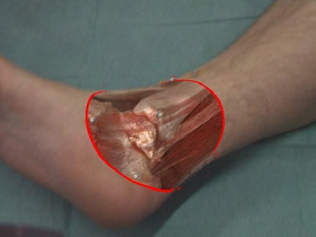
\includegraphics[width=\textwidth]{image/AR_in_medicine}
			\caption{استفاده از واقعیت افزوده در پزشکی
			\\
		\cite{nasir}}
			\label{fig:gull}
		\end{subfigure}
		~ %add desired spacing between images, e. g. ~, \quad, \qquad, \hfill etc. 
		%(or a blank line to force the subfigure onto a new line)
		\begin{subfigure}[b]{0.4\textwidth}
			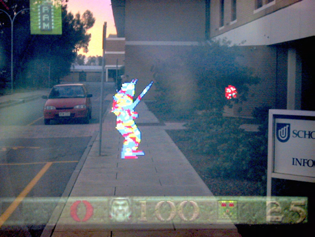
\includegraphics[width=\textwidth]{image/ARQuake_outdoor_AR_game}
			\caption{استفاده از واقعیت افزوده برای بازی
			\\
			\cite{serino2016pokemon}}
			\label{fig:tiger}
		\end{subfigure}
		~ %add desired spacing between images, e. g. ~, \quad, \qquad, \hfill etc. 
		%(or a blank line to force the subfigure onto a new line)
		
		\begin{subfigure}[b]{0.4\textwidth}
			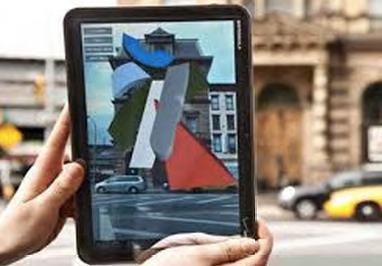
\includegraphics[width=\textwidth]{image/AR_architecture_by_Re+Public}
			\caption{استفاده از واقعیت افزوده در مهندسی
			\\
			\cite{Fjeld}}
			\label{fig:mouse}
		\end{subfigure}
		\caption{انواع استفاده از واقعیت افزوده}\label{fig:َARType}
	\end{figure}
در شکل \ref{fig:َARType} نمونه های مختلفی از استفاده واقعیت افزوده را می‌توان مشاهده نمود.
\section{تاریخچه}
گرچه واقعیت افزوده امروزه محبوب شده است، اما این فنّاوری جدید نیست، برای هزاران سال مردم از آینه‌ها، منابع نوری و ... برای ایجاد تصاویر مختلف در دنیای واقعی استفاده می‌کردند. برای مثال در قرن ۱۷ ام تئاترها و موزه‌ها از آینه‌های متعددی  برای ادغام انعکاس اجسام و افزودن تصویری مجازی به دنیای واقعی استفاده می‌کردند\cite{Brooker}.

ایوان ساترلند  \LTRfootnote{Ivan Sutherland} اولین کسی بود که با استفاده از رایانه‌ها در دانشگاه ام آی تی \LTRfootnote{Massachusetts Institute of Technology} و در سال ۱۹۶۳ توانست تصاویر مجازی را به دنیای واقعی بیاورد\cite{Sutherland}.نمونه‌ای از پروژه انجام شده توسط ساترلند را در شکل \ref{fig:Sutherland1968} می‌بینیم. او در سال ۱۹۶۸ به دانشگاه هاروارد \LTRfootnote{Harvard University} رفت و در آنجا با کمک باب اسپرول \LTRfootnote{Bob Sproull } توانستند اولین دستگاه واقعیت افزوده را بسازند\cite{Sutherland2}. این دستگاه بر روی سر قرار می‌گرفت و با استفاده از تابش نور بر روی عدسی‌ای مقابل چشمان سعی بر آن داشت تا تصاویر مفهومی را به بیننده نمایش دهد. برای ایجاد تصاویر ۳ بعدی از چندین عدسی و با استفاده از تابش‌های مختلف در جهات مختلف، توانستند تصاویر ۳ بعدی را بسازند\cite{Sutherland2}.

\begin{figure}
	\centering
	\begin{subfigure}[b]{0.3\textwidth}
		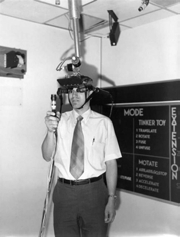
\includegraphics[width=\textwidth]{image/s2}
		
		\label{fig:gull}
	\end{subfigure}
	~ %add desired spacing between images, e. g. ~, \quad, \qquad, \hfill etc. 
	%(or a blank line to force the subfigure onto a new line)
	\begin{subfigure}[b]{0.6\textwidth}
		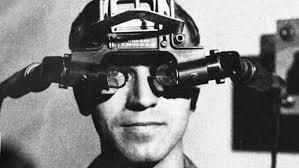
\includegraphics[width=\textwidth]{image/s1}
		
		\label{fig:tiger}
	\end{subfigure}
	~ %add desired spacing between images, e. g. ~, \quad, \qquad, \hfill etc. 
	%(or a blank line to force the subfigure onto a new line)
	
	\caption{سیستم واقعیت افزوده طراحی شده توسط ساترلند ، ۱۹۶۸ \cite{Sutherland2}}\label{fig:Sutherland1968}
\end{figure}

در سال‌های بعد، تحقیق بر روی این فنّاوری علاوه بر دانشگاه‌ها، در آزمایشگاه‌های نظامی و دولتی نیز شروع شد و موردتوجه قرار گرفت. به‌عنوان‌ مثال تام فورنس\LTRfootnote{Tom Furness} در آزمایشگاه‌های هوا و قضای آمریکا، بر روی این فنّاوری شروع به تحقیق نمود و پروژه ای با نام سوپر کاکپیت \LTRfootnote{Super-Cockpit}را شروع کرد که به آموزش خلبانان هواپیما کمک می‌کرد\cite{Furness}.در شکل \ref{fig:airforce1} نمونه‌ای از این آزمایش را می‌بینیم.

\begin{figure}
	\centering
	\begin{subfigure}[b]{0.4\textwidth}
		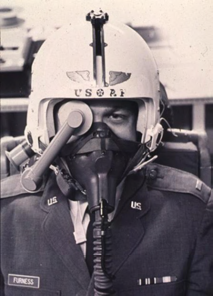
\includegraphics[width=\textwidth]{image/airforce1}
		\caption{دوربین نصب شده بر روی سر یک خلبان}
		\label{fig:airforce1}
	\end{subfigure}
	~ %add desired spacing between images, e. g. ~, \quad, \qquad, \hfill etc. 
	%(or a blank line to force the subfigure onto a new line)
	\begin{subfigure}[b]{0.5\textwidth}
		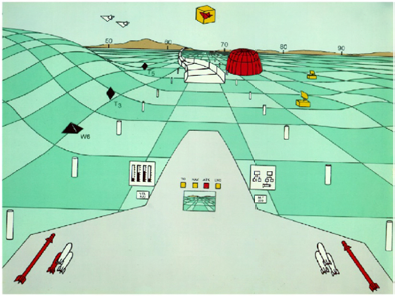
\includegraphics[width=\textwidth]{image/airforce2}
		\caption{تصویر شبیه سازی شده در پروژه}
		\label{fig:tiger}
	\end{subfigure}
	~ %add desired spacing between images, e. g. ~, \quad, \qquad, \hfill etc. 
	%(or a blank line to force the subfigure onto a new line)
	
	\caption{پروژه سوپر کاکپیت \cite{Furness2}}\label{fig:Super-Cockpit}
\end{figure}


در سال ۱۹۸۱ آژانس ملی فضا و هواشناسی \LTRfootnote{National Aeronautics and Space Administration (NASA)} شروع به تحقیق بر روی این فنّاوری نمود و کلاه و نمایشگر مخصوص به خود را نیز طراحی کرد که می‌توانست برای آموزش فضانوردان با ایجاد تصاویر مجازی کمک بکند\cite{Furness2}.

\section{انگیزه پژوهش}
\noindent
گارتنر\LTRfootnote{Gartner}، شرکت پژوهشی و مشاوره آمریکایی است، که درزمینه ارائه خدمات برون‌سپاری، تحقیق و پژوهش و مشاوره فناوری اطلاعات فعالیت می‌نماید. شرکت گارتنر در سال ۱۹۷۹ توسط گارتنر گیدون \LTRfootnote{Gideon Gartner} راه‌اندازی شد و در حال حاضر دارای عملیات در ۸۵ کشور جهان است. دفتر مرکزی این شرکت در شهر استنفورد، کنتیکت، ایالات‌متحده آمریکا قرار دارد و سهام آن در بازار بورس نیویورک معامله می‌شود\LTRfootnote{https://en.wikipedia.org/wiki/Gartner}.

این شرکت هرساله نموداری را معرفی می‌کند که در آن به معرفی تکنولوژی‌های روز پرداخته و موقعیت آنها آن‌ها را بررسی می‌کند\LTRfootnote{https://www.gartner.com/smarterwithgartner/5-trends-emerge-in-gartner-hype-cycle-for-emerging-technologies-2018/}.شکل:\ref{fig:gartner}
\\

\begin{figure}[tb]
	\centering
	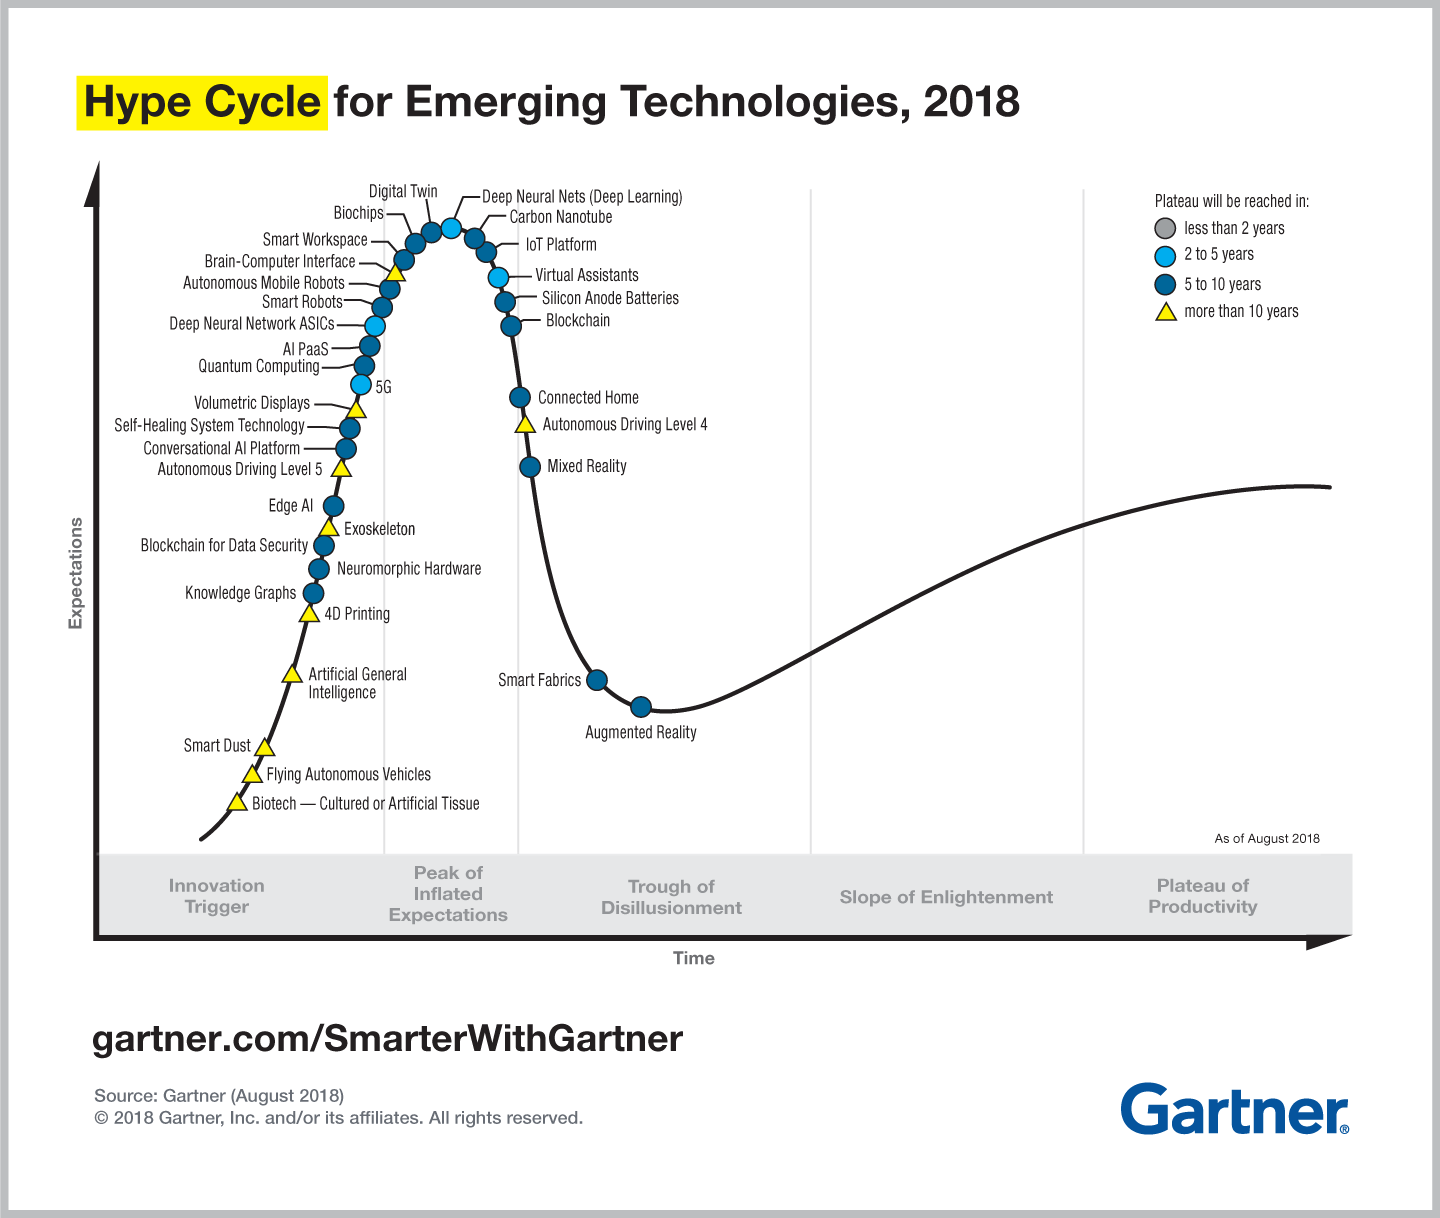
\includegraphics[width=1\linewidth]{image/gartner}
	\caption {نمودار موقعیت فنّاوری‌ها در سال ۲۰۱۸\cite{gartner}}
	\label{fig:gartner}
\end{figure}
\noindent
این نمودار از ۵ قسمت مختلف تشکیل‌شده است: 
\\
\textbf{
	۱-راه افتادن فنّاوری \LTRfootnote{Technology Trigger} : }در این مرحله یک فنّاوری مفهوم‌سازی می‌شود، پتانسیل‌های آن موردبررسی قرار می‌گیرد و شروع به اثبات ادعاهای خود می‌کند.
\\
\textbf{
	۲-اوج انتظارات \LTRfootnote{Peak of Inflated Expectations} : }در این مرحله تکنولوژی به پیاده‌سازی می‌رسد و نظریات و تبلیغات در رابطه با موفقیت‌آمیز بودن و یا نبودن آن مطرح می‌شود.
\\
\textbf{
	۳-مرحله سرخوردگی \LTRfootnote{Trough of Disillusionment} :} در این مرحله مشکلات تکنولوژی نمایان می‌شود و شروع تلاش‌ها برای رفع این مشکلات است.
\\
\textbf{
	۴-شیب روشنگری \LTRfootnote{Slope of Enlightenment} :} در این مرحله شرکت‌های مختلف به این تکنولوژی روی می‌آورند و پتانسیل‌های این فنّاوری برای آینده نمایان‌تر می‌شود.
\\
\textbf{
	۵-فلات بهره‌وری \LTRfootnote{Plateau of Productivity} :} در اینجا استفاده از این فناوری گسترده و همه‌گیر شده و تعداد خیلی زیادی از شرکت‌های کوچک و بزرگ به آن روی می‌آورند.

همان‌طور که ملاحظه می‌شود این فنّاوری در مرحله سوم قرار دارد و مشکلاتی دارد که باعث می‌شود زمینه خوبی برای مطالعه و تحقیق باشد و همچنین بسیار گرایش برای آن وجود دارد به‌طوری‌که شرکت بزرگی مانند گارتنر این فنّاوری را پیشنهاد می‌دهد و پیش‌بینی می‌کند که یکی از فنّاوری‌هایی باشد که در آینده نزدیک شاهد ظهور و گسترده شدن آن خواهیم بود.

یکی از مراجع مهم و معروف برای مقاله‌ها در این زمینه، نشست بین‌المللی واقعیت افزوده و واقعیت ترکیبی ایسمار\LTRfootnote{International Symposium on Mixed and Augmented Reality (ISMAR)} است که در قالب "نشست رایانه‌ای آی ای ای ای" \LTRfootnote{IEEE Computer Society } به‌صورت سالیانه برگزار می‌شود، با بررسی و ارزیابی دو دهه از مقاله‌های منتشرشده در این کنفرانس، به نمودارهای زیر می‌رسیم‌\RTLfootnote{در این مقاله منظور از \lr{Rendering} نحوه پردازش تصویر است و با واژه رندرینگ در این تحقیق متفاوت است. }\cite{ismar}.
\begin{figure}
	\centering
	\begin{subfigure}[b]{1\textwidth}
		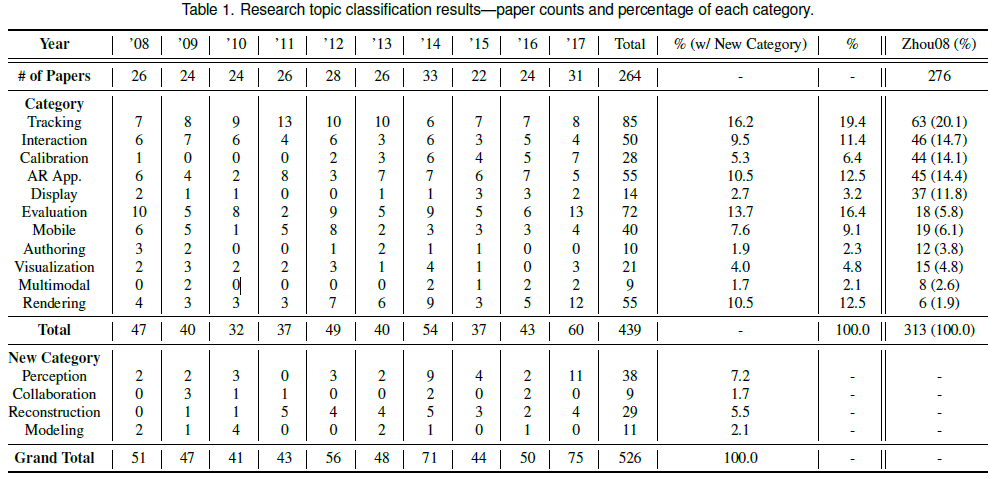
\includegraphics[width=\textwidth]{image/ismar1}
		\caption{تعداد مقاله ها بر اساس موضوع}
		\label{fig:gull}
	\end{subfigure}
	~ %add desired spacing between images, e. g. ~, \quad, \qquad, \hfill etc. 
	%(or a blank line to force the subfigure onto a new line)
	\begin{subfigure}[b]{0.4\textwidth}
		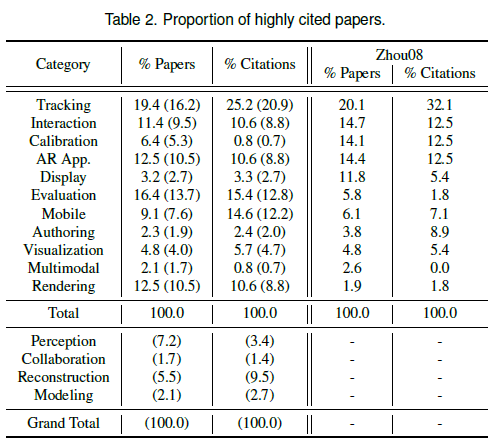
\includegraphics[width=\textwidth]{image/ismar2}
		\caption{ارجاع به مقالات به نسبت تعداد}
		\label{fig:tiger}
	\end{subfigure}
	~ %add desired spacing between images, e. g. ~, \quad, \qquad, \hfill etc. 
	%(or a blank line to force the subfigure onto a new line)
	\begin{subfigure}[b]{0.5\textwidth}
		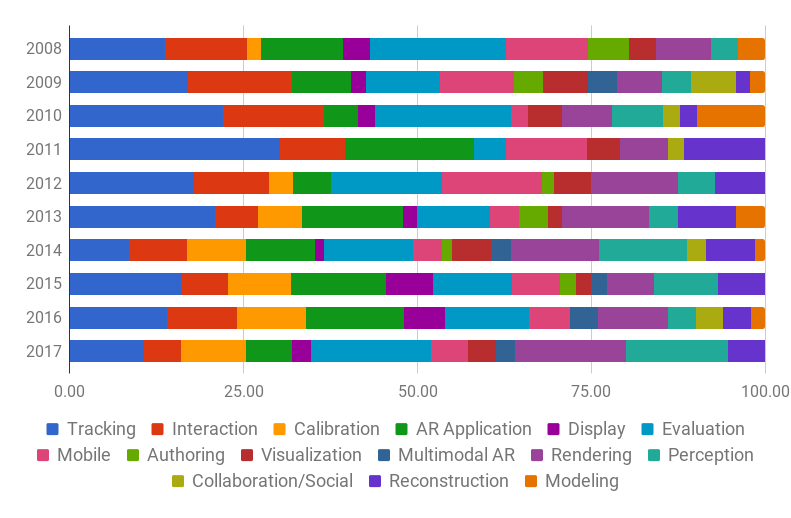
\includegraphics[width=\textwidth]{image/ismar3}
		\caption{مقابسه تمایل نویسندگان بر اساس موضوع}
		\label{fig:tiger}
	\end{subfigure}
\begin{subfigure}[b]{0.5\textwidth}
	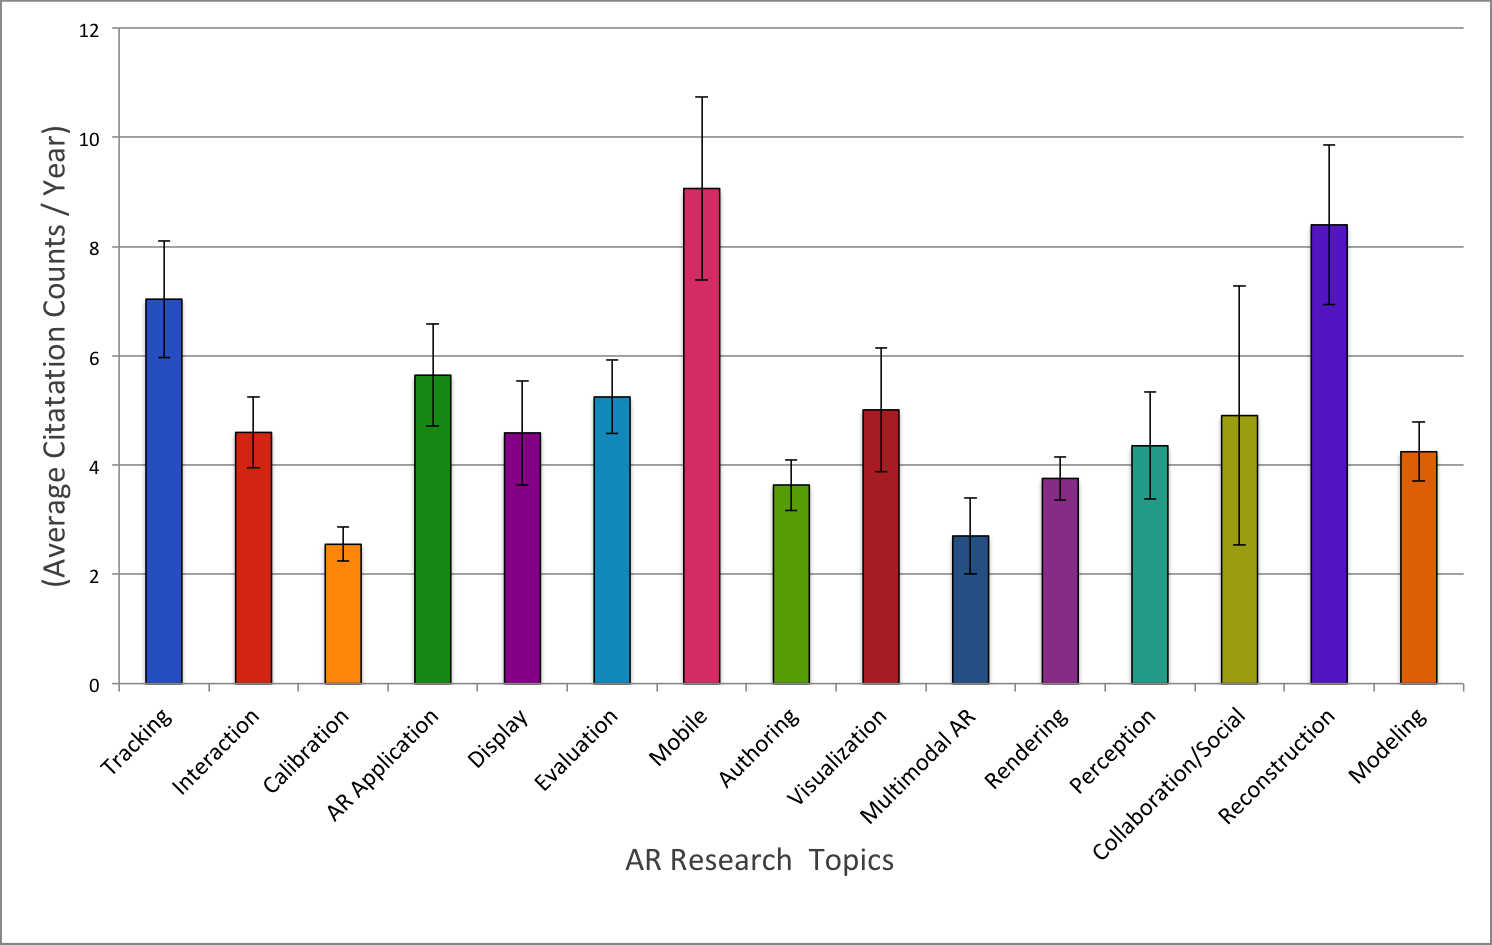
\includegraphics[width=\textwidth]{image/ismar4}
	\caption{میانگین ارجاع به مقالات در سال بر اساس موضوع}
	\label{fig:tiger}
\end{subfigure}
	\caption{بررسی 2 دهه کنفرانس ISMAR\cite{ismar}}\label{fig:ISMAR}
\end{figure}

 همان‌طور که از نتایج شکل \ref{fig:ISMAR} پیدا است یکی از حوزه‌های موردعلاقه محققین ردیابی\LTRfootnote{Tracking}، است که مقاله‌های زیادی در این حوزه منتشر می‌شود و همچنین ارجاعات به این مقالات نیز بالا می‌باشد.در نتیجه، این تحقیق اهمیت این موضوع و باز بودن جای کار در این حوزه را نشان می‌دهد.



\section{بیان ساختار فصل‌های بعدی}
بخش‌بندی سمینار به شکل زیر است:
\\
\textbf{
	بخش دوم:} در این بخش درخت موضوعی را به نمایش می‌گزاریم، ادبیات موضوع را مطرح کرده، کلیه اطلاعات لازم در واقعیت افزوده را شرح داده و به بیان حوزه‌های مختلف در آن می‌پردازیم و به‌اختصار آن‌ها را شرح می‌دهیم.
\\
\textbf{
	بخش سوم: } در این بخش به معرفی رندرینگ در واقعیت افزوده می‌پردازیم و اجزای آن را شرح می‌دهیم و سپس تمرکز خودمان را بر روی ردیابی (Tracking) می‌گزاریم و روش‌های مختلف درون آن را شرح می‌دهیم و کارهای گذشته را ذکر می‌کنیم و با یک دیگر مقایسه می‌کنیم.
\\
\textbf{
	فصل چهارم:} در این فصل روش‌های مختلف را باهم مقایسه کرده و مسئله‌ای را مطرح می‌کنیم و به اهمیت این مسئله می‌پردازیم و راه حل‌های احتمالی در رابطه با مسئله را بیان می‌کنیم.


\cchapter{ادبیات تحقیق}
\section{مقدمه}
در این فصل به ارائه مفاهیم پایه می‌پردازیم و مفاهیمی که  باید خواننده با آن‌ها آشنا باشد تا بتواند به‌مرور فصل‌های بعدی بپردازد و دچار سردرگمی خواننده نشود را بیان می‌کنیم.

در ابتدا به معرفی واقعیت افزوده می‌پردازیم سپس انواع رابط‌های کاربری و حوزه‌های مشابه با واقعیت افزوده را شرح می‌دهیم. در زیر بخش بعدی انواع دستگاه‌های واقعیت افزوده را معرفی می‌کنیم و با یکدیگر مقایسه می‌کنیم و در زیر بخش بعد به معرفی انواع روش‌های دریافت ورودی در این سیستم و تعامل با کاربر می‌پردازیم.در بخش آخر نیز در رابطه با نمایشگرها و شیوه کاری آن‌ها صحبت می‌کنیم آن‌ها را با یکدیگر مقایسه می‌کنیم.
\section{معرفی}
\subsection{انواع رابط کاربری}
\noindent
محقق آزوما\LTRfootnote{Ron Azuma} بیان می‌کند که واقعیت افزوده باید شامل ۳ ویژگی باشد\cite{Azuma}:
\\
۱- باید توانایی ترکیب دنیای واقعی و مجازی را دارا باشد.
\\
۲- باید با دنیای واقعی در ارتباط باشد.
\\
۳- باید به‌صورت ۳ بعدی قابل استناد باشد.
\\
مثال شبکه خبری سی ان ان هر سه این شرایط را دارا می‌باشد. تصویر مجازی خبرنگار جسیکا یلین به‌صورت زنده بر روی صحنه ظاهر شد و همچنین توانایی برقراری ارتباط و صحبت با خبرنگار ولف بلیتزر در همان زمان بود و تصویر مجازی به‌صورت سه بعدی قابل‌نمایش بود.

در یک سیستم واقعیت افزوده هر سه شرط باید رعایت شود و همچنین باید شامل یک سیستم کامپیوتری که قادر است تصاویر مجازی تولید کند و به دنیای واقعی اضافه کند باشد، همچنین باید یک سیستم ردیابی \LTRfootnote{Tracking} را دارا باشد تا بتواند نقطه مناسب برای ظاهر شدن تصویر مجازی را شناسایی بکند و تصویر مجازی را بر روی آن به نمایش درآورد. در قسمت بعدی این تحقیق مفصل به بیان سیستم ردیابی می‌پردازیم.

باید توجه شود که در تعریف آزوما هیچ محدودیتی آورده نشده در مورد نوع تکنولوژی که برای ظاهر کردن تصاویر در دنیای واقعی از آن استفاده می‌کنیم، همچنین در سیستم لزومی به‌ظاهر شدن تصویر نمی‌باشد و می‌تواند به پخش موسیقی و یا پخش فیلم بپردازد.

اگر با یک دید جامع نگاه بکنیم، واقعیت افزوده آخرین تلاش توسط محققین و مهندسین برای حذف رابط کاربری در کامپیوترها و افزایش تعامل کاربر با دنیای واقعی است.ریکامتو\LTRfootnote{Rekimoto}  تفاوت بین رابط‌های میز کار سنتی \LTRfootnote{traditional desktop computer interfaces} با تلاش‌هایی که در جهت حذف رابط کاربری انجام‌شده است را متمایز ساخت\cite{Rekimoto}. همان‌طور که در شکل \ref{fig:Rekimoto} قابل‌مشاهده است، ریکامتو به معرفی انواع رابط‌های کاربری پرداخت و ۴ مدل را معرفی نمود.
\\
\begin{figure}[tb]
	\centering
	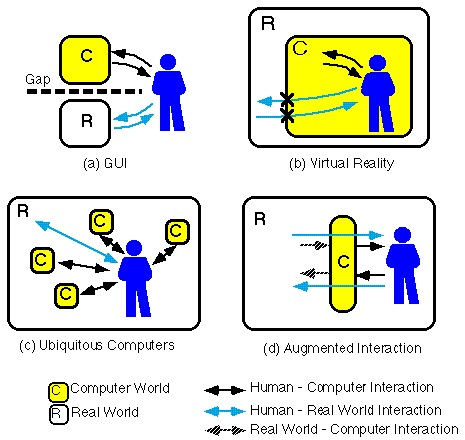
\includegraphics[width=1\linewidth]{image/style}
	\caption {انواع رابط‌های کاربری\cite{Rekimoto}}
	\label{fig:Rekimoto}
\end{figure}
\textbf{1- مدل رابط گرافیکی کاربر \lr{(GUI)}:\LTRfootnote{graphical user interface}}در این مدل کاربر با استفاده از اشکال گرافیکی که توسط کامپیوتر در اختیارش قرار می‌گیرد ارتباط برقرار می‌کند مانند آیکون‌ها، محیط ویندوز، منوها و ...
\\
\textbf{
	۲- مدل واقعیت مجازی:\LTRfootnote{Virtual Reality} }در این مدل کاربر با استفاده از کلاهی که بر روی سر و چشمانش قرار می‌گیرد وارد دنیای مجازی شده و درون این دنیا قرار می‌گیرد و با استفاده از دستکش‌ها و یا دسته‌های مخصوص شروع به تعامل با دنیای مجازی می‌کند و به‌اصطلاح درون این دنیا غواصی\LTRfootnote{immersive} می‌کند و از دنیای واقعی جدا می‌شود.
\\
\textbf{۳ -مدل پردازش همه‌جا حاضر:\LTRfootnote{Ubiquitous Computing} }در این مدل سنسورها و پردازشگرها در دنیای واقعی جاسازی‌شده‌اند.
\\
\textbf{
	۴- واقعیت افزوده:\LTRfootnote{Augmented Reality}} مشکل مدل دوم (واقعیت مجازی) این است که کاربر از دنیای واقعی جداشده و توانایی ارتباط با آن را ندارد ولی در این مدل کاربر علاوه بر توانایی تعامل با دنیای مجازی، قادر است با دنیای واقعی نیز تعامل بکند و این دو نه‌تنها مشکلی برای هم ایجاد نمی‌کنند، بلکه مکمل و کمک‌کننده به یکدیگر هستند.

همان‌طور که در تعاریف بالا می‌توانیم ببینم، رابطه نزدیکی بین واقعیت مجازی و واقعیت افزوده وجود دارد، همچنین هر دو آن‌ها دارای صفحه‌نمایشی که بر روی سر نصب‌شده\LTRfootnote{head mounted displays}، سیستم ردیابی و دستگاه‌های ورودی دستی\LTRfootnote{handheld input devices} می‌باشند، بااین‌حال بین این دو تفاوت‌های مهمی وجود دارد.

هدف اصلی از واقعیت مجازی، استفاده از تکنولوژی برای جایگزینی آن با دنیای واقعی است و در مقابل آن در واقعیت افزوده، تکنولوژی سعی بر آن دارد  با استفاده از محتوای دیجیتال\LTRfootnote{digital content} بدون آنکه به کاربر حس غوطه‌ور شدگی دست بدهد به دنیای واقعی بیفزاید. در واقعیت مجازی دستگاه نمایشگر باید کاملاً جامع باشد و میدان گسترده‌ای از دید را پوشش بدهد و گرافیک‌های ۳ بعدی تا حد امکان واقعی به نظر بیایند. ازآنجاکه کاربر به مدت زیادی قادر به دیدن دنیای واقعی نمی‌باشد، در واقعیت مجازی سیستم ردیابی نیاز به دقیق بودن به نسبت دنیای واقعی را ندارد و این حساسیت در آن کمتر می‌باشد.

در مقابل، در  واقعیت افزوده، سیستم نمایش می‌تواند به‌صورت غیر غوطه‌ور کننده، با گستردگی دید کم و با استفاده از گرافیک‌های کوچک باشد. ولی در اینجا، سیستم ردیابی باید بسیار دقیق باشد و توانایی داشته باشد تا محتوای مجازی را دقیقاً بر روی دنیای واقعی قرار بدهد. برای کاربران واقعیت افزوده بسیار ساده است تا متوجه چندین میلی‌متر تفاوت قرار گرفتن محتوای مجازی با دنیای واقعی بشوند.

\subsection{واقعیت ترکیبی}
برای توضیح بیشتر برای واقعیت افزوده می‌توانیم به نتیجه تحقیق میلگرام\LTRfootnote{Milgram} و کشینو\LTRfootnote{Kishino} نگاهی بیندازیم\cite{Milgram}. آنها مفهومی با نام واقعیت ترکیبی\LTRfootnote{Mixed Reality} را معرفی نمودند که این مفهوم دو مفهوم واقعیت و مجازی را با یکدیگر ترکیب می‌کند و همچنین طبقه‌بندی‌هایی را بر اساس میزان ترکیب مجازی و واقعیت بیان می‌کند. در سمت راست محیط مجازی\LTRfootnote{Virtual Environment} را می‌بینیم، جایی که دید کاربر از جهان توسط کامپیوترهایی که تصاویر مجازی تولید می‌کنند کاملاً جایگزین شده است. در سمت مخالف، یعنی در سمت چپ ما شاهد محیط واقعی\LTRfootnote{Real Environment} هستیم که در آن کاربر هیچ‌گونه دید و درکی از عناصر مجازی ندارد و کاملاً درون دنیای واقعی قرارگرفته است. هر چه از محیط واقعی به سمت محیط مجازی حرکت کنیم، میزان عناصر مجازی در دید کاربر افزایش میابد و این محیط مابین، به دو دسته دیگر تقسیم می‌شوند. دسته واقعیت افزوده که در آن میزان واقعیت در دید کاربر خیلی بیشتر از مجازی است و دسته مجازی افزوده‌شده\LTRfootnote{Augmented Virtuality} که درون آن، بیشتر دید کاربر را عناصر مجازی تشکیل داده است و قسمت کمی را عناصر واقعی تشکیل می‌دهند.

با استفاده از شکل \ref{fig:Mixed}، به این نتیجه می‌رسیم که واقعیت افزوده خود به‌تنهایی به‌عنوان دسته مجزا شناخته نمی‌شود بلکه بخشی از هر دو را تشکیل می‌دهد.

\begin{figure}[!ht]
	\centering
	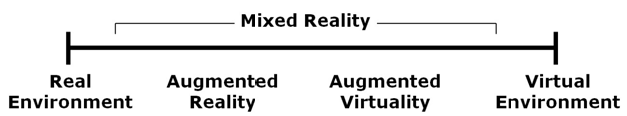
\includegraphics[width=1\linewidth]{image/mixedreality}
	\caption {شکل معرفی شده برای واقعیت ترکیبی توسط میلگرام\cite{Milgram}}
	\label{fig:Mixed}
\end{figure}

\section{انواع دستگاه‌های واقعیت افزوده}

دستگاه‌های نمایشگری که با استفاده از آن‌ها تکنولوژی واقعیت افزوده را به نمایش درمی‌آوریم به سه دسته کلی تقسیم می‌شوند\cite{Julie}:
\\
\subsection{نمایشگرهایی که بر روی سر نصب می‌شوند}
 این نوع از نمایشگرها بر روی سر قرار می‌گیرند\protect\LTRfootnote{head mounted displays (HMD)} مانند کلاه ایمنی و یا مانند عینک، در جلوی چشمان قرار داده می‌شوند و  قادر هستند هر دو تصویر از دنیای مجازی و واقعی را بر روی‌هم قرار داده و به کاربر نشان بدهند.در شکل \ref{fig:hmd} می‌توانیم نمونه‌ای از این دستگاه‌ها را ببینیم
	. این دستگاه‌ها به دو صورت کار می‌کنند.
\begin{itemize}
	\item \textbf{1- دیدن از طریق ویدیو\LTRfootnote{Video-see-through}:} در این مدل، نیاز داریم تا کاربر، ۲ دوربین را بر روی سرخود قرار دهد و با استفاده از پردازش‌های تصاویر این دو دوربین، تصاویر ۳ بعدی از محیط را  به‌صورت زنده دریافت کنیم و همزمان با استفاده از یک کامپیوتر، تصاویر ۳ بعدی مجازی را طراحی بکنیم و با تصاویر دریافتی از دوربین‌ها، ادغام بکنیم، در این روش به دو مشکل برخورد می‌کنیم، مشکل اول کیفیت تصاویر است که وابسته به‌وضوح \LTRfootnote{resolution} دوربین‌ها و پردازشگرهای تصاویر است و همچنین وابسته به کیفیت تصویر تولیدشده توسط کامپیوتر است و مشکل بعدی این است که باید سرعت کارها در این نوع بالا باشد تا تأخیر \LTRfootnote{latency}دریافت تصاویر و پردازش و سپس نمایش را به حداقل برسانیم.
	\item \textbf{
		2- دیدن از طریق نور:\LTRfootnote{optical-see-through} }در این مدل کاربر با استفاده از لنزها، قادر است دنیای واقعی را ببیند، و با استفاده از دستگاه‌های خاص و تابش نور به لنزها، تصاویر ۳ بعدی را برای کاربر طراحی می‌کنیم. در اینجا کیفیت تصاویر دریافتی به نسبت روش قبل بالاتر است زیرا برای دیدن دنیای واقعی نیازی به‌وضوح نمایشگر نداریم ولی برای ایجاد کردن تصاویر ۳ بعدی در این روش مشکل است. همچنین به دلیل اینکه تصاویر محیط واقعی را بدون واسطه دریافت می‌کنیم، تأخیر در اینجا نیز کمتر از روش قبلی است.
\end{itemize}

\begin{figure}[tb]
	\centering
	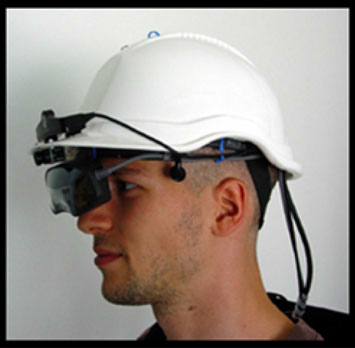
\includegraphics[width=0.6\linewidth]{image/hmd}
	\caption {نمونه‌ای از نمایشگرهای نصب‌شده بر روی سر\cite{Julie}}
	\label{fig:hmd}
\end{figure}

\subsection{نمایشگرهای دستی}
نمایشگرهای دستی\LTRfootnote{Handheld displays}، با کمک گرفتن از دستگاه‌های محاسباتی کوچک که دارای نمایشگر می‌باشند کار می‌کنند و برای ادغام کردن تصاویر مجازی با دنیای واقعی از روش "دیدن از طریق ویدئو" استفاده می‌کنند. به‌عنوان‌مثال برای این نوع از نمایشگرها می‌توان تلفن‌های  همراه هوشمند را مثال زد که علاوه بر دارا بودن ویژگی‌های ذکرشده، دارای سنسورهایی مانند "سیستم موقعیت یاب جهانی"\LTRfootnote{Global Positioning System (GPS)} و قطب نمای دیجیتال هستند که برای ردیابی می‌توان از آن‌ها استفاده نمود. در شکل \ref{fig:mobile} می‌توانیم نمونه‌ای از این دستگاه‌ها را ببینیم.

\begin{figure}[tb]
	\centering
	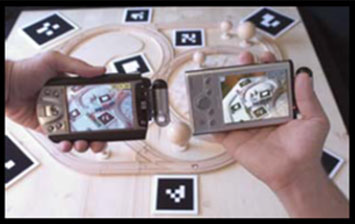
\includegraphics[width=0.7\linewidth]{image/mobile}
	\caption {نمونه‌ای از نمایشگرهای دستی\cite{Julie}}
	\label{fig:mobile}
\end{figure}
\subsection{نمایشگرهای فضایی}
در این نوع از نمایشگرها ما شاهد واقعیت افزوده فضایی\LTRfootnote{Spatial Augmented Reality (SAR)} هستیم که با استفاده از ویدئو پروژکتور، عناصر نوری، هولوگرام‌ها و برچسب‌های فرکانس رادیویی به‌صورت مستیم عناصر مجازی را به درون دنیای واقعی میاورند و دیگر کاربر نیازی ندارد که دستگاهی را بر روی سرخود قرار بدهد و یا اینکه دستگاهی را حمل بکند شکل\ref{fig:sar}. در نمایشگرهای فضایی\LTRfootnote{spatial displays}، بیشتر فنّاوری بدون وابستگی به کاربر است و بدون دخالت او، عناصر مجازی را با روش اضافه کردن مستقیم\LTRfootnote{direct
	augmentation} با دنیای واقعی ادغام می‌کنیم\cite{Bimber}.
\begin{figure}[tb]
	\centering
	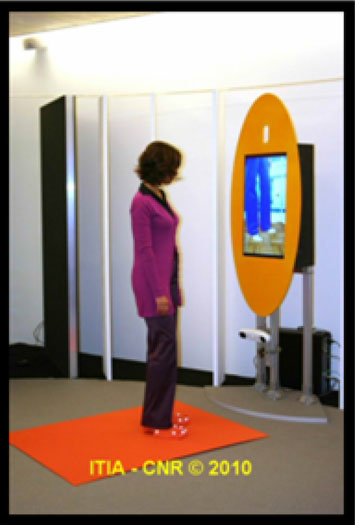
\includegraphics[width=0.6\linewidth]{image/sar}
	\caption {نمونه‌ای از نمایشگرهای فضایی\cite{Bimber}}
	\label{fig:sar}
\end{figure}
\section{ورودی و تعامل}
سیستم‌های واقعیت افزوده می‌توانند روش‌های مختلف دریافت ورودی را با یک دیگر ترکیب بکنند، مانند دریافت از صوت، دستکش‌های مخصوص، لمس کردن تصویر، پردازش تصویر و غیره. دریافت ورودی‌ها در برنامه‌های مختلف با توجه به نیاز هر برنامه متفاوت است.
سیستم‌های طراحی‌شده برای دریافت ورودی و تعامل با واقعیت افزوده را می‌توان به ۵ دسته زیر تقسیم نمود:

\subsection{مرورگرهای اطلاعات}
مرورگرهای اطلاعات\LTRfootnote{Information Browsers} رابطی است برای نشان دادن اطلاعات واقعیت افزوده بر روی دنیای واقعی. این نوع از دریافت اطلاعات و تعامل، نماینده‌ای از برنامه‌های واقعیت‌های افزوده است و درجایی کار می‌کنند که نمایشگر واقعیت افزوده به‌عنوان پنجره‌ای به‌سوی فضای اطلاعاتی در نظر گرفته می‌شود و وظیفه اصلی کاربر این است که این پنجره را کنترل کرده تا بتواند اطلاعات را دریافت بکند. اولین نمونه از این برنامه "ناوی کم"\LTRfootnote{NaviCam} شکل \ref{fig:navicam} است که بر روی گوشی‌های هوشمند پیاده‌سازی شد. این نوع از برنامه‌ها نیاز به انجام تعامل‌های پایه دارد و شیوه کار آن‌ها به این صورت است که صحنه واقعیت افزوده را پردازش می‌کنند و اطلاعات برای کاربر پردازش می‌شود \cite{Rekimoto}.
\begin{figure}[tb]
	\centering
	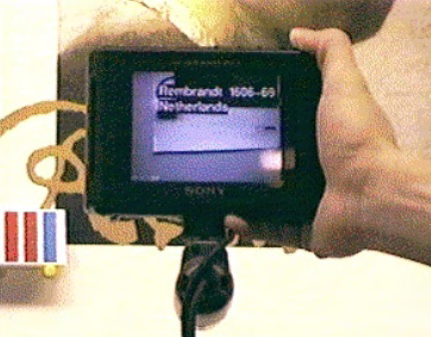
\includegraphics[width=0.6\linewidth]{image/navicam}
	\caption {نمونه‌ای از پروژه ناوی کم\cite{Rekimoto}}
	\label{fig:navicam}
\end{figure}
\subsection{رابط کاربر ۳ بعدی}
در مدل رابط کاربر 3 بعدی\LTRfootnote{3D User Interfaces} با استفاده از تکنیک‌های تعاملی ۳ بعدی به ارتباط با محتوا در فضا می‌پردازیم. این روش یکی از راه‌های جذاب و مناسب برای تعامل است. "بومن"\LTRfootnote{Bowman} به‌طور خلاصه این فرایند را به سه قسمت تقسیم کرده است\cite{Bowman}.
\begin{itemize}
	\item 
	\textbf{
		جهت‌یابی\protect\LTRfootnote{navigation}: }در این قسمت نیاز است که عنصر ۳ بعدی دیده شود و در اصل به سمت آن جهت‌یابی شویم، این قسمت بسیار ساده است و با حرکات بدن کاربر قابل پیاده‌سازی است. در بسیاری از دستگاه‌ها کاربر می‌تواند در سه بعد حرکت کند و در هر سه جهت نیز بچرخد.
	\item 
	\textbf{
		انتخاب\LTRfootnote{selection}:} در این قسمت نیاز است تا کاربر بتواند برای تعامل، عنصر مجازی را انتخاب بکند، برای این قسمت می‌توان از دستگاه‌های مختلف مانند سنسورها، جوی استیک\LTRfootnote{joysticks} و... استفاده کرد.
	\item 
	\textbf{
		دست‌کاری\LTRfootnote{manipulation}:} این قسمت گام آخر است و کاربر می‌تواند تعامل خود را با عناصر مجازی به‌راحتی انجام دهد.
\end{itemize}
در شکل \ref{fig:Bowman} نمونه‌ای از استفاده از رابط کاربری ۳ بعدی را می‌توان مشاهده نمود.
\begin{figure}[tb]
	\centering
	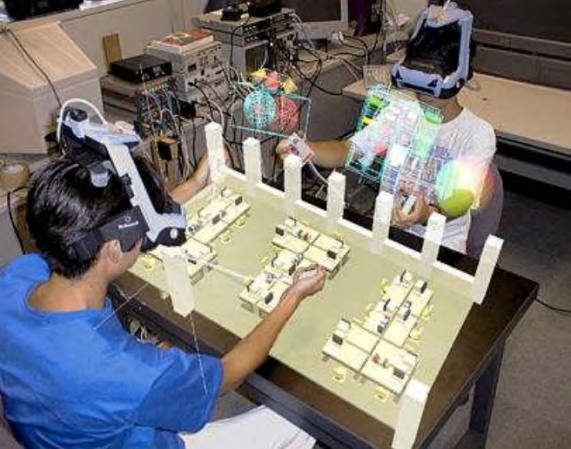
\includegraphics[width=0.6\linewidth]{image/3d}
	\caption {استفاده از رابط کاربر ۳ بعدی \cite{Bowman}}
	\label{fig:Bowman}
\end{figure}
\subsection{رابط کاربر قابل‌ لمس}
در رابط کاربر قابل‌ لمس\LTRfootnote{Tangible User Interfaces} از رابط‌ها، برای ارتباط با عناصر مجازی از عناصر دنیای واقعی استفاده می‌کنیم. این اجسام مانند پلی بین دنیای واقعی و دنیای مجازی می‌باشند و تعامل را برقرار می‌سازند. این روش یکی از روش‌های نوین برای تعامل با دنیای مجازی است، اما مشکلات خود را نیز دارا است، به‌عنوان‌مثال، وقتی‌که قصد داریم یک عنصر مجازی را بر روی عنصر فیزیکی به وجود بیاوریم، این عنصر مجازی یا باید با استفاده از پرتو تابیده شود، و یا بر روی نمایشگر کاربر ظاهر شود، در این رابط، ممکن است فاصله‌ای بین جسم مجازی و فیزیکی به وجود بیاید که ناخوشایند است\cite{Kato}.در شکل \ref{fig:tar} نمونه‌ای از استفاده از رابط کاربر قابل لمس را می‌توان مشاهده نمود.

\begin{figure}[tb]
	\centering
	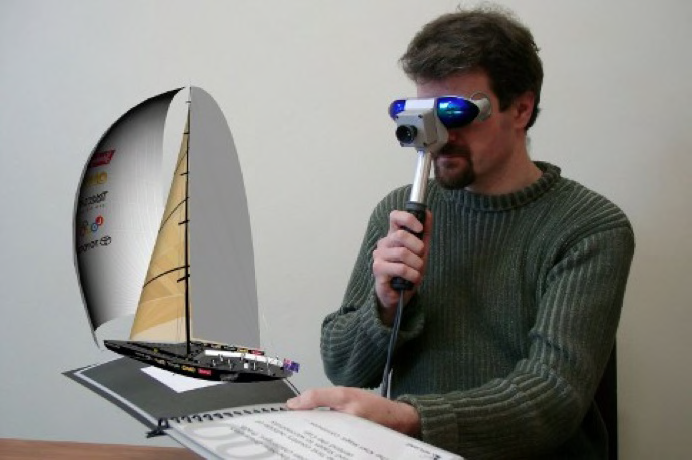
\includegraphics[width=0.6\linewidth]{image/tar}
	\caption {استفاده از رابط کاربر قابل لمس \cite{Kato}}
	\label{fig:tar}
\end{figure}
\subsection{رابط کاربر طبیعی}
در مدل رابط کاربر طبیعی\LTRfootnote{Natural User Interfaces} از اجزای طبیعی بدن مانند دست‌ها استفاده می‌کنیم، در این حالت اجزای بدن می‌توانند ردیابی شوند و تشخیص داده شوند با استفاده از سنسورهای مختلفی که کاربر می‌تواند پوشیده باشد. سنسورهای مختلفی در اندازه‌ها و شکل‌های مختلفی برای این کار ساخته‌شده‌اند.
با پیشرفت کامپیوترها، سیستم‌های واقعیت افزوده توانستند حرکت و ژست بدن کاربر را بدون نیاز به سنسورها تشخیص بدهند. به‌طور مثال لی\LTRfootnote{Lee} توانست سیستمی را طراحی کند که توانایی شناسایی دست و حرکت‌های آن را داشته باشد\cite{Lee}.به طور مثال در شکل \ref{fig:lee} می‌توان روش ارائه شده توسط لی را مشاهده نمود.

\begin{figure}[!ht]
	\centering
	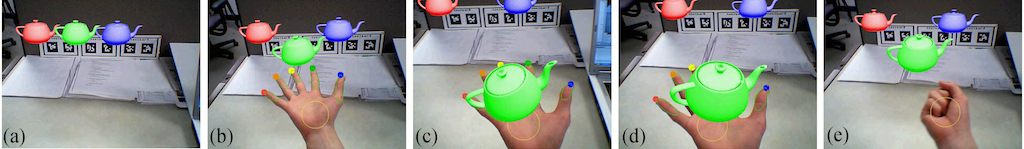
\includegraphics[height=4cm,width=1\linewidth]{image/handyar}
	\caption {استفاده از رابط کاربر طبیعی \cite{Lee}}
	\label{fig:lee}
\end{figure}

\subsection{رابط چند منظوره}
برای تعامل قوی‌تر در برنامه‌های واقعیت افزوده، محققین سعی کردند تا مدل‌های مختلفی از ورودی‌ها را با یکدیگر ترکیب کنند، در این میان ترکیب گفتار\LTRfootnote{speech} و تشخیص ژست\LTRfootnote{gesture recognition}، یکی از گسترده‌ترین و فعال‌ترین بخش‌ها بوده است.

لی در این رابطه تحقیقات زیادی انجام داد و یک سیستم چندمنظوره را طراحی کرد که در آن با استفاده از یک دوربین به  ردیابی ژست دست می‌پرداخت و همچنین با دریافت گفتار و ترکیب این دو، دستورات را شناسایی می‌کرد و به تعامل با کامپیوتر می‌پرداخت.
او توانست دقت را در این روش شناسایی کند و بیان کرد که با این ترکیب در سیستم واقعیت افزوده ۲۵ درصد سریع‌تر به نسبت تشخیص ژست به‌تنهایی، می‌توان به تعامل پرداخت\cite{Lee2}.به طور مثال  در شکل   \ref{fig:lee2} می‌توان روش ارائه شده توسط لی برای رابط چند منظوره\LTRfootnote{Multimodal Interfaces} را مشاهده نمود.

\begin{figure}[!ht]
	\centering
	\begin{subfigure}[b]{0.5\textwidth}
		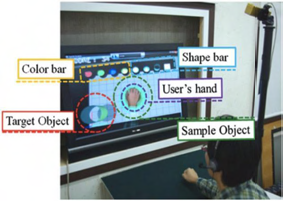
\includegraphics[width=\textwidth]{image/lee2}
		
		
	\end{subfigure}
	~ %add desired spacing between images, e. g. ~, \quad, \qquad, \hfill etc. 
	%(or a blank line to force the subfigure onto a new line)
	\begin{subfigure}[b]{0.4\textwidth}
		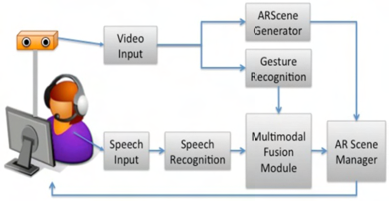
\includegraphics[width=\textwidth]{image/lee1}
		
	\end{subfigure}
	\caption{رابط چند منظوره\cite{Lee2}}\label{fig:lee2}
\end{figure}

\section{نمایش}
در واقعیت افزوده، اشیاء مجازی و دنیای واقعی باید با یکدیگر ترکیب شوند و به صورت همزمان نمایش داده
شوند. برای رسیدن به این هدف قبل از به نمایش درآمدن واقعیت افزوده چندین فرایند باید انجام شوند که
عبارتند از: کالیبره کردن دوربین\LTRfootnote{calibration}، ثبت\LTRfootnote{registration}، ردیابی و ساخت\LTRfootnote{construction}.

کالیبره کردن دوربین رویه‌ای است که در آن پارامترهای دوربین مجازی با دوربین واقعی منطبق می‌شود شکل \ref{fig:Billinghurst}. 

\begin{figure}
	\centering
	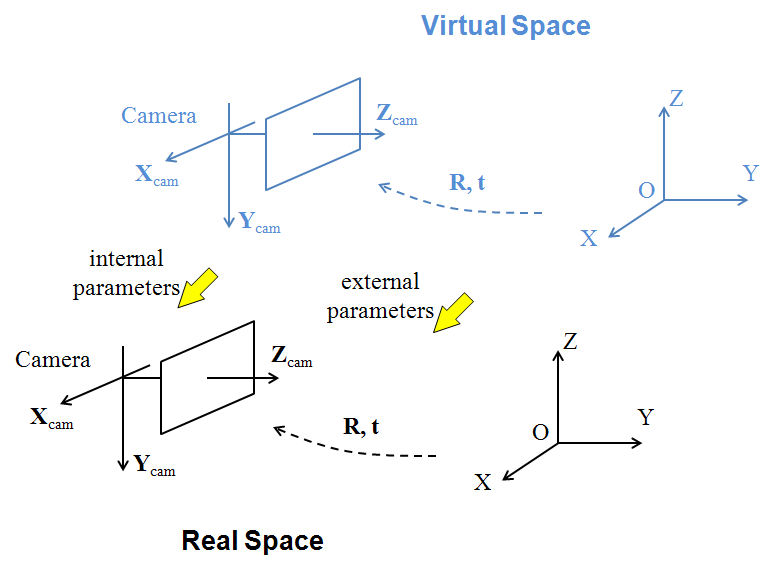
\includegraphics[width=1\linewidth]{image/realspace}
	\caption {منطبق کردن پارامترهای داخلی و خارجی \cite{Billinghurst}}
	\label{fig:Billinghurst}
\end{figure}

این امر برای نمایش صحیح اشیاء مجازی منطبق بادید کاربر، نیاز است. دوربین‌ها دارای دو نوع از پارامترها هستند، پارامترهای داخلی و پارامترهای خارجی. 

\begin{itemize}
	\item \textbf{پارامترهای داخلی، }
 پارامترهایی هستند که ساختار سه بعدی محیط را به تصویر دو بعدی تبدیل می‌کنند. پارامترهای داخلی با تهیه چندین تصویر توسط دوربین از الگوهای شناخته‌شده و مقایسه ویژگی‌های تصاویر به‌دست‌آمده از این الگوها با ویژگی‌های سه بعدی آنها، تعیین می‌شوند. این امر معمولاً قبل از شروع به‌کار سیستم واقعیت افزوده انجام می‌شود.
 \item \textbf{پارامترهای خارجی}
   با ردگیری دوربین و تعیین فاصله و جهت دوربین تعیین می‌شوند. هنگامی‌که صحنه ایستا است تنها تعیین پارامترهای خارجی دوربین در حالت اولیه کافی است ولی درصحنه‌هایی که تغییر می‌کنند به این دلیل که هر تغییری ممکن است درصحنه مجازی که قرار است به محیط واقعی اضافه شود، تغییر ایجاد کند، هر جسم مهمی که مکان آن تغییر می‌کند باید ردگیری شود\cite{Billinghurst}.
\end{itemize}
با استفاده از روش‌های ردگیری، مکان و جهت دوربین و اجسام موجود در هر صحنه مشخص می‌شود. برای آنکه صحنه مجازی به‌صورت صحیح به صحنه واقعی افزوده شود، هر صحنه مجازی باید با صحنه واقعی متناظر خود تطبیق داده شود، به این رویه، رویه ثبت گفته می‌شود. پس از تطبیق صحنه واقعی با صحنه مجازی، تصویر غنی‌شده ایجاد می‌شود که می‌تواند طبق کاربرد و فنّاوری به‌کاربرده شده به‌صورت دیجیتالی و یا به‌صورت فیزیکی نمایش داده شود.

در این بخش ابتدا به بررسی انواع فناوری‌های نمایش مورداستفاده در واقعیت افزوده و سپس ازنظر نوع نمایش و فاصله محل قرارگیری از چشم کاربر بررسی می‌شوند.
\subsection{فناوری نمایش}
فناوری‌های نمایش واقعیت افزوده بسته به نوع ترکیب تصویر مجازی با تصویر واقعی به سه دسته تقسیم می‌شوند: ویدیوئی\LTRfootnote{Video based}، دید نوری\LTRfootnote{Optical see-through} و ایجاد تصویر بر روی یک سطح فیزیکی\LTRfootnote{Projection onto a physical surface}.
\subsubsection{ویدیوئی}
در این نوع نمایش ابتدا تصویر محیط واقعی را به‌وسیله دوربین به‌صورت دیجیتالی تبدیل می‌کنند و سپس تصویر مجازی به کمک روش‌های پردازش تصویر، به تصویر محیط واقعی اضافه می‌شود. در بیشتر موارد دوربین در پشت صفحه‌نمایش متصل می‌شود و اجازه دیدمستقیم به محیط را می‌دهد. درواقع در این مدل دنیای واقعی را از طریق صفحه‌نمایش می‌بینیم. دوربین می‌تواند در زوایای دیگر نیز قرار گیرد مثلاً رو به کاربر برای ایجاد یک آینه مجازی\cite{Billinghurst}.
با رایج شدن استفاده از دوربین‌های دیجیتال در رایانه‌ها، رایانه‌های لوحی و تلفن‌های هوشمند پیاده‌سازی واقعیت افزوده به‌سادگی امکان‌پذیر شده است. این امر سبب شده تا واقعیت افزوده ویدیوئی به عمومی‌ترین نوع واقعیت افزوده تبدیل شود. همچنین باوجود دوربین‌های دیجیتال و الگوریتم‌های پیشرفته ردگیری امکان افزایش دقت ترکیب تصویر واقعی با تصویر مجازی، در حد پیکسل فراهم‌شده است. یکی از مشکلات رایج این نوع واقعیت افزوده، عدم رعایت صحیح رابطه بین اجسام واقعی و مجازی است بدین‌صورت که قسمتی از جسم واقعی که نزدیک‌تر از محل قرارگیری جسم مجازی است در زیر جسم مجازی اضافه‌شده به تصویر، قرار می‌گیرد\cite{Tian}.

همان‌طور که در شکل \ref{fig:Tian}دیده می‌شود در سمت چپ شی مجازی به‌صورت نادرستی به محیط واقعی اضافه‌شده است و این مشکل در شکل سمت راست رفع شده است. این مشکل با به‌دست آوردن اطلاعات عمقی صحنه واقعی و مقایسه این اطلاعات با اطلاعات مجازی که باید به صحنه واقعی اضافه شود قابل‌حل است. جدیدترین روش به‌دست آوردن اطلاعات عمقی محیط استفاده از روش‌های تصویر پایه است \cite{Billinghurst}.
بدین‌صورت که با مقایسه دو تصویر و ترکیب آنها اطلاعات عمقی محیط به‌دست می‌آید. از دیگر روش‌های به‌دست آوردن عمق محیط استفاده از دوربین‌های پیمایش عمقی است که همراه با تصویر رنگی یک نقشه از اطلاعات عمقی محیط را نیز فراهم می‌کنند.
\begin{figure}
	\centering
	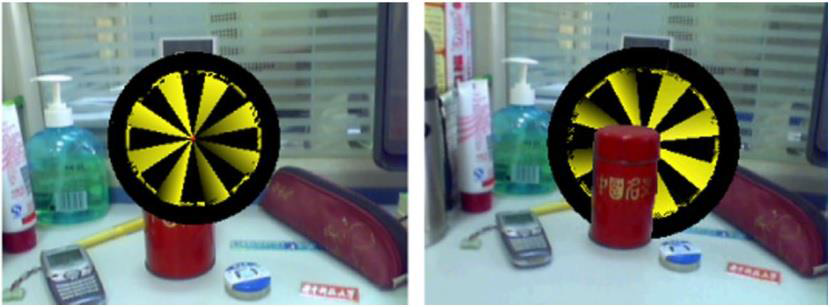
\includegraphics[width=1\linewidth]{image/wrongpic}
	\caption {اضافه شدن اشتباه در شکل سمت چپ و تصحیح آن در سمت راست \cite{Tian}}
	\label{fig:Tian}
\end{figure}


اصلی‌ترین مشکل واقعیت افزوده ویدیوئی، دید غیرمستقیم (از طریق نمایشگر) از محیط است \cite{Billinghurst}، تصویری که از طریق دوربین تهیه‌شده است دارای چندین محدودیت مانند وضوح و کیفیت تصویر، جابجایی چشم و تأخیر است. این کاستی‌ها در کاربردهایی مانند پزشکی که دیدمستقیم از محیط نیاز است بسیار مهم می‌شوند.

از دیگر مشکلات این نوع نمایش، نیاز بالای قدرت پردازشی است. باوجود افزایش قدرت پردازشی در سال‌های اخیر، در مقایسه با دیگر انواع نمایش واقعیت افزوده هنوز نیاز به افزایش قدرت پردازش در این نوع واقعیت افزوده هست.

\subsubsection{دید نوری}
این نوع از واقعیت افزوده از سیستم‌های نوری برای نمایش تصویر مجازی به همراه تصویر محیط واقعی استفاده می‌کنند. این سیستم‌ها معمولاً از جداکننده نور\LTRfootnote{beam splitters (e.g. half mirrors or combined prisms)} استفاده می‌کنند. این جداکننده تصویر واقعی را با انعکاس تصویر مجازی ترکیب کرده و نمایش می‌دهد شکل\ref{fig:optical}. بتصویر مجازی ترکیب کرده و نمایش می‌دهد شکل. بیشتر این نوع از سیستم‌ها از ملحق کننده نور، جدا از صفحه‌نمایش برای ترکیب دنیای واقعی و تصویر مجازی استفاده می‌کنند. اخیراً با پیشرفت فنّاوری صفحه‌نمایش‌هایی ساخته‌شده که شفاف هستند، استفاده از آنها در واقعیت افزوده به‌شدت روبه افزایش است. استفاده از این نوع صفحه‌نمایش‌ها باعث سادگی و کوچک شدن ساختار سیستم دید نوری واقعیت افزوده می‌شود\cite{Billinghurst}.

\begin{figure}
	\centering
	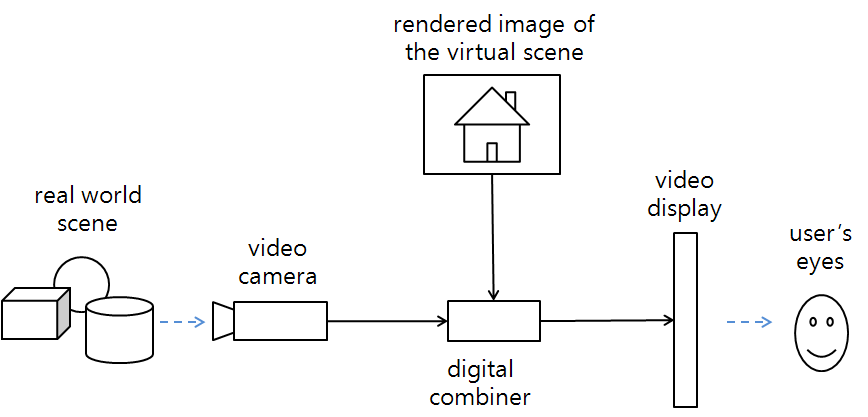
\includegraphics[width=1\linewidth]{image/opticalview}
	\caption {نمایش دید نوری \cite{Billinghurst}}
	\label{fig:optical}
\end{figure}

یکی از مهم‌ترین برتری‌هایی که این روش نسبت روش ویدیوئی دارد ایجاد دیدمستقیم از محیط واقعی است. با این امکان این نوع از واقعیت افزوده از مشکلاتی مانند تأخیر، کم بودن وضوح و غیره رنج نمی‌برد و برای کاربردهایی مناسب است که به دیدمستقیم از دنیای واقعی نیاز دارند مانند کاربردهای پزشکی و نظامی که این‌یک ویژگی بسیار مهم است.

اصلی‌ترین مشکل این نوع از واقعیت افزوده دقت پایین در نگاشت دو تصویر محیط واقعی و مجازی بر روی یکدیگر است. در بیشتر پیاده‌سازی‌ها نیاز به کالیبره کردن رویه ثبت است که معمولاً دقت پایین‌تری نسبت به رویه‌های خودکار موجود در واقعیت افزوده ویدیوئی دارند. به این دلیل که پارامترهای کالیبره کردن تصاویر واقعی و مجازی به نسبت زیادی وابسته به فضای بین چشم کاربر و صحنه موردنظر است و این فضا در طول زمان تغییر می‌کند و باعث ایجاد خطا در نگاشت دو تصویر واقعی و مجازی بر یکدیگر می‌شود \cite{Billinghurst}.

یکی دیگر از مشکلات واقعیت افزوده دید نوری تأخیر موقتی بین نمایش تصویر مجازی و دیده مستقیم واقعی است. باوجود سیستم ردگیری دقیق بازهم یک تأخیر موقتی بین نمایش تصویر مجازی و دید دنیای واقعی وجود دارد.

در بسیاری از موارد، ایجاد رابطه صحیح عمقی بین دنیای واقعی و مجازی در واقعیت افزوده دید نوری مشکل است. با توجه به ماهیت نیمه شفاف ترکیب‌کننده تصاویر، کاربران یک دید نیمه شفاف از تصویر دنیای واقعی و مجازی دارند. به‌صورتی که، هیچ‌کدام دیگری را تماماً نمی‌پوشاند. کیاکاوا\LTRfootnote{Kiyokawa} و همکاران\cite{Kiyokawa} برای رفع این مشکل یک ماسک الکترونیکی برای پوشاندن مکان‌هایی که اشیاء مجازی اضافه می‌شوند طراحی کرد. با بستن پیکسل‌هایی از صفحه‌نمایش که اشیای مجازی در آن پیکسل‌ها قرار می‌گیرند دید دنیای واقعی بسته‌شده و اشیاء مجازی واضح‌تر به نمایش درمی‌آیند.

شرایط نوری محیط می‌تواند در دید واقعیت افزوده دید نوری تأثیرگذار باشد. در اکثر مواقع ترکیب‌کننده نوری دارای شفافیت ایستا است که می‌تواند باعث خطا در میزان روشنایی تصویر مجازی و دید محیط واقعی شود. در محیط‌های بیرونی اشیاء مجازی باید تیره‌تر از تصویر محیط واقعی به نمایش درآیند. برای رفع این مشکل نمایشگرهای متصل به سر به چندین کاور با میزان شفافیت متفاوت مجهز شده‌اند.
\subsubsection{نمایش مبتنی بر نورپردازی}
واقعیت افزوده مبتنی بر نورپردازی سطح یک جسم واقعی را به کمک نورپردازی با تصویر مجازی می‌پوشاند شکل\ref{fig:tajmahal}. با توجه به ترکیب ردگیری زاویه دید کاربر و سطح فیزیکی اجسام، واقعیت افزوده مبتنی بر نورپردازی دارای قابلیت اضافه کردن تعاملی را دارد\cite{Raskar}. در بیشتر مواقع برای این منظور از ویدئو پروژکتور متصل به سقف و یا دیوار برای پوشاندن سطح اجسام استفاده می‌شود. این امر سبب می‌شود که قابلیت جابجایی وجود نداشته باشد و محدود به مکانی باشد که پروژکتور می‌تواند نورپردازی کند. البته در سال‌های اخیر تلاش‌هایی برای ایجاد قابلیت جابجایی برای ویدئو پروژکتورها شده است که می‌توان به نمونه‌هایی که قابلیت قرار گرفتن در دست\cite{Mistry} و متصل شدن به سر است\cite{krum2012augmented} اشاره کرد.

\begin{figure}
	\centering
	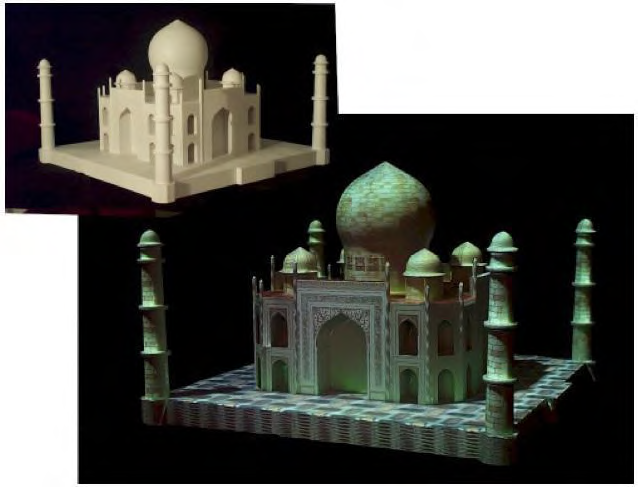
\includegraphics[width=1\linewidth]{image/tajmahal}
	\caption {نمایش دید نوری \cite{Mistry}}
	\label{fig:tajmahal}
\end{figure}

یکی از محدودیت‌های واقعیت افزوده مبتنی بر نورپردازی، نیازمند بودن به سطح یک جسم برای نمایش تصویر مجازی است که باعث می‌شود تنها اجسام نزدیک به پروژکتور مناسب باشند و در استفاده برای کاربردهای شهری محدودیت ایجاد می‌کند. همچنین این نوع از واقعیت افزوده وابستگی بیشتری به شرایط نوری محیط دارد چراکه سایه دیگر اجسام می‌تواند مشکل‌ساز باشد. همچنین ایجاد رابطه صحیح عمقی بین سطح جسم موردنظر و دیگر اجسام مشکل است.

%\subsection{فاصله قرار گیری نمایشگر}
%یکی دیگر از جنبه‌های نمایش واقعیت افزوده فاصله نمایشگر از چشم کاربر است که می‌توانند در دسته‌هایی مانند نمایشگر متصل به سر\LTRfootnote{Head-attached Displays}، نمایشگر دستی و یا متصل به بدن\LTRfootnote{Handheld and Body-attached Displays} و نمایشگر فاصله‌دار\LTRfootnote{Spatial Displays} قرار گیرند.
%
%	
%
%\subsubsection{نمایشگر متصل به سر}
%این نوع نمایشگر تصویر مجازی را درست در جلوی چشمان کاربر نمایش می‌دهد، که در این صورت جسم دیگری مانع دیدن تصویر نمی‌شود. این نوع نمایشگرها در اندازه‌های مختلف وجود دارند که از اندازه یک کلاه تا اندازه یک عینک متفاوت است. به همان نسبت که حمل و متصل کردن آن به سر راحت‌تر می‌شود، تصویر عریض‌تر و درخشان‌تر می‌شود\cite{Billinghurst}.
%\subsubsection{نمایشگر دستی و یا متصل به بدن}
%نمایشگر متصل به سر دارای قابلیت‌هایی مانند قابلیت حمل بالا و فراهم کردن تصویر فراگیر است اما به دلیل پوشیدنی بودن آنها در بعضی از موارد دارای محدودیت هستند. نمایشگرهای در دست گرفتنی و یا متصل به بدن به‌عنوان نمایشگرهای شخصی و قابل‌حمل در نظر گرفته می‌شوند و در صورت نیاز قابل به اشتراک‌گذاری با دیگران هستند. آنها همچنین ازنظر اجتماعی قابل پذیرش تر از نمایشگر متصل به سر هستند.
%
%با پیشرفت فنّاوری درزمینه دستگاه‌های قابل‌حمل، قدرت پردازشی دستگاه‌های قابل‌حمل برای پردازش تصویرسازی واقعیت افزوده به میزان لازم افزایش پیداکرده است. اخیراً آزمایش‌هایی برای استفاده از سنسورهای عمقی بر روی رایانه‌های لوحی و تلفن‌های هوشمند انجام‌شده است (مانند پروژه تانگو گوگل.) \protect\LTRfootnote{https://developers.google.com/tango} نمایی از این پروژه در شکل \ref{fig:tango} آمده است.
%
%
%\begin{figure}
%	\centering
%	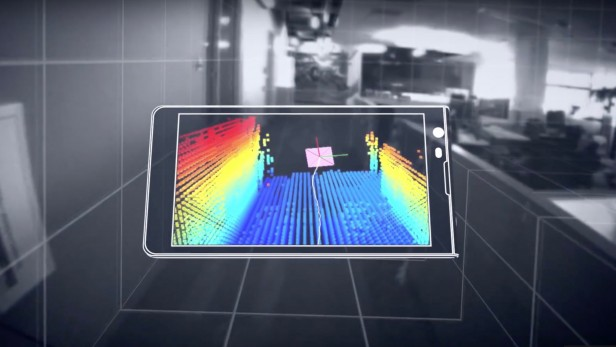
\includegraphics[width=1\linewidth]{image/tango}
%	\caption {پروژه تانگو گوگل که با استفاده زا نمایشگرهای دستی کار می‌کند}
%	\label{fig:tango}
%\end{figure}
%\subsubsection{نمایشگر فاصلهای}
%این نوع از نمایشگر در مقایسه با دو نوع قبلی قابلیت حمل کمتری دارد و معمولاً در یک مکان ثابت نصب می‌شود. به این دلیل که این نوع نمایشگرها دارای اندازه بزرگی هستند. درنتیجه، برای استفاده در مکان‌های عمومی و کاربردهایی که چندین کاربر دارند مناسب هستند. از نمونه‌های این نوع نمایشگر می‌توان به نمایشگرهای رومیزی که با یک دوربین در تماس هستند اشاره کرد. از دیگر نمونه‌های آن ساخت آینه مجازی است که از یک نمایشگر بزرگ و یک دوربین رو به کاربر تشکیل‌شده است و تصویر کاربر به همراه اطلاعات مجازی اضافه‌شده در آن نمایش داده می‌شود\cite{Billinghurst}.
\section{رندرینگ به چه معنا است؟}
در حوزه واقعیت افزوده، ۳ واژه بسیار مهم وجود دارد به نام ردیابی\LTRfootnote{Tracking}، کالیبراسیون\LTRfootnote{Calibration} و ثبت\LTRfootnote{Registration} که زیرمجموعه رندریگ\LTRfootnote{Rendering} می‌باشند و در کنار هم به این واژه معنا می‌دهند. این ۳ واژه همیشه همراه هم هستند و در یک هدف قرار دارند. برای ثبت پویا\LTRfootnote{dynamic}، نیاز به داشتن ردیابی هستیم. عناصر درون سیستم واقعیت افزوده ثبت می‌شوند و سپس در یک سیستم هماهنگ، این عناصر ثبت‌شده به دنیای واقعی پیوند\LTRfootnote{aligned} می‌شوند. در واقعیت افزوده هدف اصلی این است که اطلاعات مجازی دقیقاً به‌صورتی که از قبل برنامه‌ریزی‌شده‌اند، ثبت بشوند. کالیبراسیون به‌صورت دقیق اطلاعات حس‌گرها\LTRfootnote{sensor} را دریافت و پردازش می‌کند و مسئولیت ثبت ایستا\LTRfootnote{Static} با این فرایند است\cite{siltanen2012theory}. در شکل \ref{fig:rct} می‌توانیم روابط بین ثبت، کالیبراسیون و ردیابی را در کنار هم و به صورت نمادین ببینیم.


\begin{figure}
	\centering
	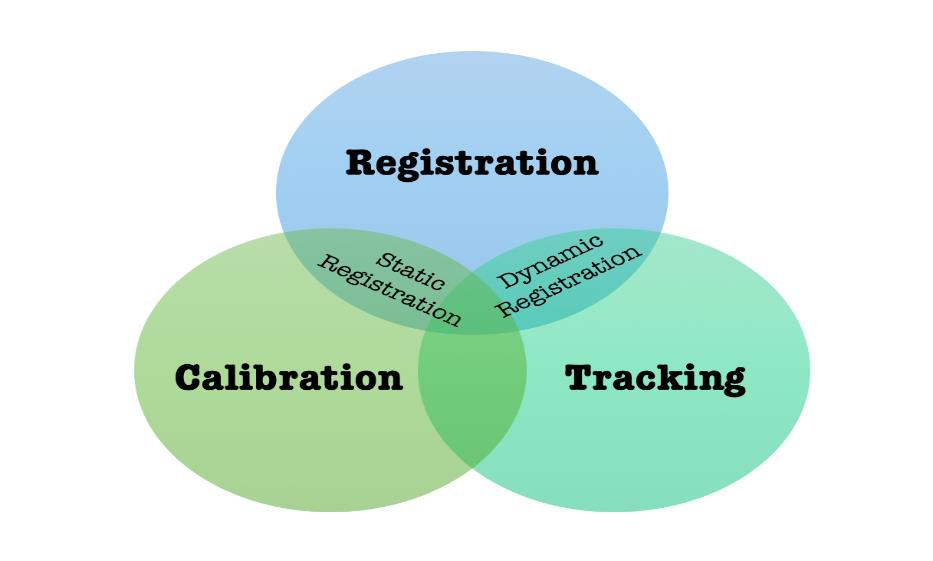
\includegraphics[width=1\linewidth]{image/rct}
	\caption {ارتباط ثبت، ردیابی و کالیبراسیون\cite{siltanen2012theory}}
	\label{fig:rct}
\end{figure}

ردیابی واژه‌ای است که برای حس کردن و محاسبه کردن مقادیر در واقعیت افزوده به‌کار می‌رود. برای تبدیل کردن موقعیت در ۳ بعد عناصر مجازی، به موقعیت‌های نسبی، نیاز به جهت‌یابی داریم. واقعیت افزوده به‌صورت بلادرنگ کار می‌کند درنتیجه برای ارسال مقدار از محیط واقعی باید به‌صورت بلادرنگ\LTRfootnote{real time} عمل کرد و همین‌طور این کار باید پیوسته در زمان صورت بگیرد. ردیابی درون سیستم‌های رایانه‌ای برای اجسام ۲ بعدی کاری رایج است اما سختی کار در اینجا ردیابی در محیط بیرون و در سه جهت مختصات برای همه‌ی نوع‌های عناصر است\cite{siltanen2012theory}.

به عملیات مقایسه کردن مقادیر بین دو دستگاه، کالیبراسیون گفته می‌شود. یکی بین دستگاه مرجع\LTRfootnote{reference} و دیگری بین دستگاهی که نیاز دارد اطلاعات کالیبره شده را دریافت بکند. مختصاتی که از محیط واقعی میدانیم را به دستگاه مرجع می‌دهیم  . برخلاف ردیابی که باید به‌صورت پیوسته انجام شود، عملیات کالیبراسیون در بخش‌های مختلف زمانی و به‌صورت گسسته انجام می‌شود و برای هر دستگاه فقط یک بار این کار صورت می‌گیرد مگر اینکه دستگاه دچار مشکل بشود. کیفیت کاری دستگاه‌های واقعیت افزوده وابستگی زیادی به عملیات کالیبراسیون دارد\cite{siltanen2012theory}.

به فرایند پیوند زدن مختصات عناصر مجازی با واقعی، ثبت میگوییم. به‌طور مشخص نمایشگر واقعیت افزوده باید باکیفیت بالا، عناصر مجازی را نشان دهد و یا اینکه به عناصر واقعی پیوند بزند. برای این کار نیاز داریم تا عملیات ردیابی به‌صورت کامل کار خود را انجام دهد. اگر موقعیت دوربین ثابت باشد، ما فقط با عملیات ثبت و کالیبراسیون می‌توانیم مختصات بین عناصر مجازی و واقعی را تشخیص بدهیم ولی اگر دوربین خاصیت جابه‌جایی داشته باشد، ما به عملیات ردیابی نیز، نیاز داریم\cite{siltanen2012theory}.
برای آوردن عناصر مجازی به دنیای واقعی، نیاز به یک لنگر\LTRfootnote{anchor} داریم که باید ژست (جهت\LTRfootnote{position} و موقعیت\LTRfootnote{orientation)}) آن مشخص باشد، این لنگر باید متعلق به دنیای واقعی باشد و می‌تواند شکل‌های مختلفی به خود بگیرد، به‌عنوان‌مثال می‌تواند یک منبع مغناطیسی باشد، یا نشانگر تصویر کاغذی\LTRfootnote{paper image marker} و یا موقعیت جغرافیایی که بر اساس سیستم موقعیت‌یاب جهانی تشخیص داده می‌شود.

وابسته به نوع فنّاوری که استفاده می‌شود پروسه ثبت می‌تواند به یکی و یا هر دو فاز زیر تقسیم شود.


\textbf{فاز ثبت:}
در این فاز، ژست عنصری که در حال مشاهده است با توجه به دنیای واقعی مشخص می‌شود.

\textbf{فاز ردیابی:}
در این فاز، ژست عنصری که در حال مشاهده آن هستیم را به‌صورت نسبی اندازه‌گیری می‌کنیم.

در این بخش مطابق با اصطلاحات رایج از کلمه ردیابی برای هر دو فاز استفاده می‌کنیم و در ادامه روش‌های رایج برای ردیابی که در جهت ثبت استفاده می‌شود را بیان می‌کنیم.


\cchapter{کارهای مرتبط}
\section{معرفی فصل}
همان‌طور که در شکل \ref{fig:tree} می‌بینیم، ما درخت موضوعی برای واقعیت افزوده را درآوردیم و در بخش دوم به بیان عناصر آن پرداختیم.
واقعیت افزوده را به همراه مثال‌های آن در بخش‌های اول و دوم بررسی کردیم، سپس انواع دستگاه‌هایی که می‌توان بر روی آن‌ها واقعیت افزوده را پیاده‌سازی کرد معرفی کردیم و مختصر روش‌های تعامل و دریافت ورودی در این سیستم را بررسی کردیم و همچنین انواع روش‌های نمایش در این سیستم را طبقه‌بندی کرده و روش کار را شرح دادیم.

همان‌طور که در بخش دوم اشاره شد، محقق آزوما بیان می‌کند که واقعیت افزوده باید ۳ ویژگی داشته باشد\cite{Azuma}:
\\
۱- باید توانایی ترکیب دنیای واقعی و مجازی را دارا باشد.
\\
۲- باید با دنیای واقعی در ارتباط باشد.
\\
۳- باید به‌صورت ۳ بعدی قابل استناد باشد.
\\
برای شرط سوم، باید سیستم واقعیت افزوده ما قابلیت ثبت شدن\LTRfootnote{registration} به‌صورت ۳ بعدی را دارا باشد به معنای دیگر باید بتواند به‌صورت جزئی از دنیای واقعی به نظر بیاید. در این بخش ‌بر روی فنّاوری که این نیاز را برطرف می‌کند تمرکز می‌کنیم.
\begin{figure}
	\centering
	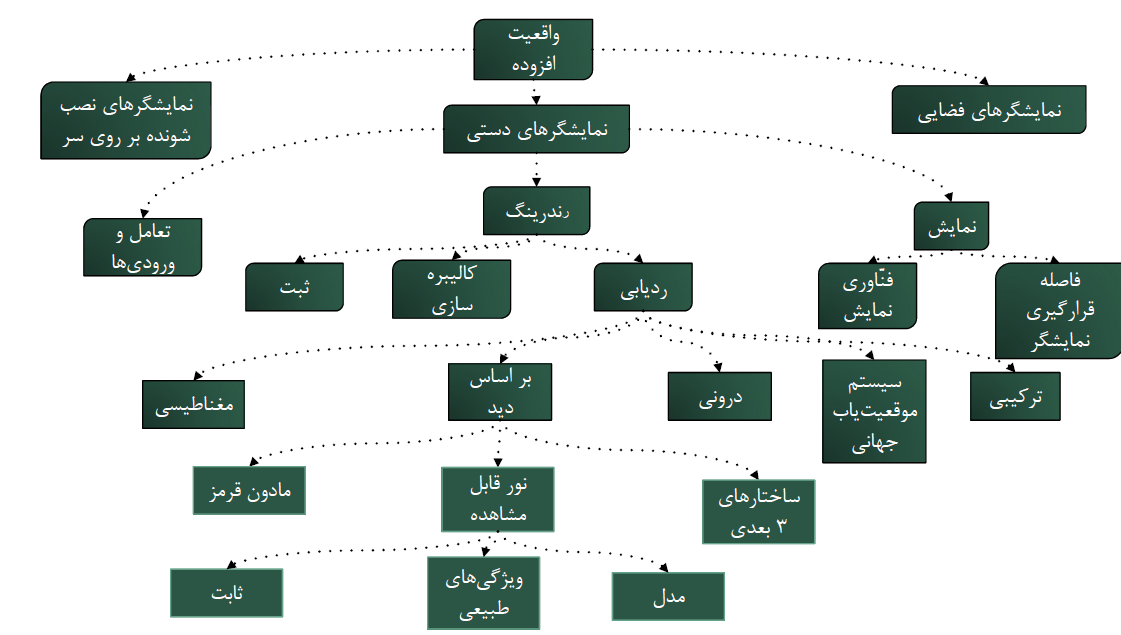
\includegraphics[height=12cm,width=1\linewidth]{image/tree}
	\caption {درخت موضوعی مربوط به واقعیت افزوده}
	\label{fig:tree}
\end{figure}

\section{ردیابی مغناطیسی}
ردیابی مغناطیسی\LTRfootnote{Magnetic Tracking} از خواص میدان‌های مغناطیسی به‌منظور محاسبه ژست یک گیرنده  که به‌عنوان یک لنگر در دنیای واقعی شناخته می‌شوند، با توجه به فرستنده استفاده می‌کند. در این مدل، فرستنده یک میدان مغناطیسی را به‌صورت متناوب تولید می‌کند که توسط یک و یا چند حسگر این اطلاعات دریافت می‌شود. با محاسبه قطب\LTRfootnote{polarization} و گرایش\LTRfootnote{orientation} میدان مغناطیسی دریافت شده، ژست دریافت‌کننده با سرعت بالایی قابل‌محاسبه است.

زمانی که از این معیار در سیستم واقعیت افزوده استفاده می‌کنیم، ردیاب مغناطیسی فرستنده به‌عنوان منشأ سیستم مختصات مجازی عمل می‌کند، و با نصب کردن یک دریافت‌کننده در عنصری که سعی در دیدن آن داریم، موقعیت و جهت آن قابل‌محاسبه است\cite{lhachemi2019augmented}. 

ردیاب‌های مغناطیسی نرخ بروز رسانی بالایی دارند و همچنین دریافت‌کننده آن‌ها کوچک و سبک هستند. ولی باید توجه داشت که قدرت میدان مغناطیسی با مکعب فاصله رابطه عکس دارد و همچنین دقت آن با توان ۴ فاصله رابطه عکس دارد. همچنین ردیابی مغناطیسی دارای معایب دیگری نیز می‌باشد مثلاً مستعد نوسان اندازه‌گیری\LTRfootnote{measurement jitter} است و نسبت به مواد مغناطیسی و میدان‌های الکتریکی در محیط واقعی حساس است.

شکل\ref{fig:magnetic} نشان‌دهنده وضوح در ردیابی مغناطیسی دستگاه‌های شرکت پولهموس\LTRfootnote{Polhemus} است که تأثیر فاصله بین دریافت‌کننده و فرستنده را نمایش می‌دهد. همان‌طور که قابل‌مشاهده است در فاصله‌های پایین این خطا بسیارکم است اما با افزایش فاصله به‌صورت نمادی خطا افزایش میابد.
\begin{figure}
	\centering
	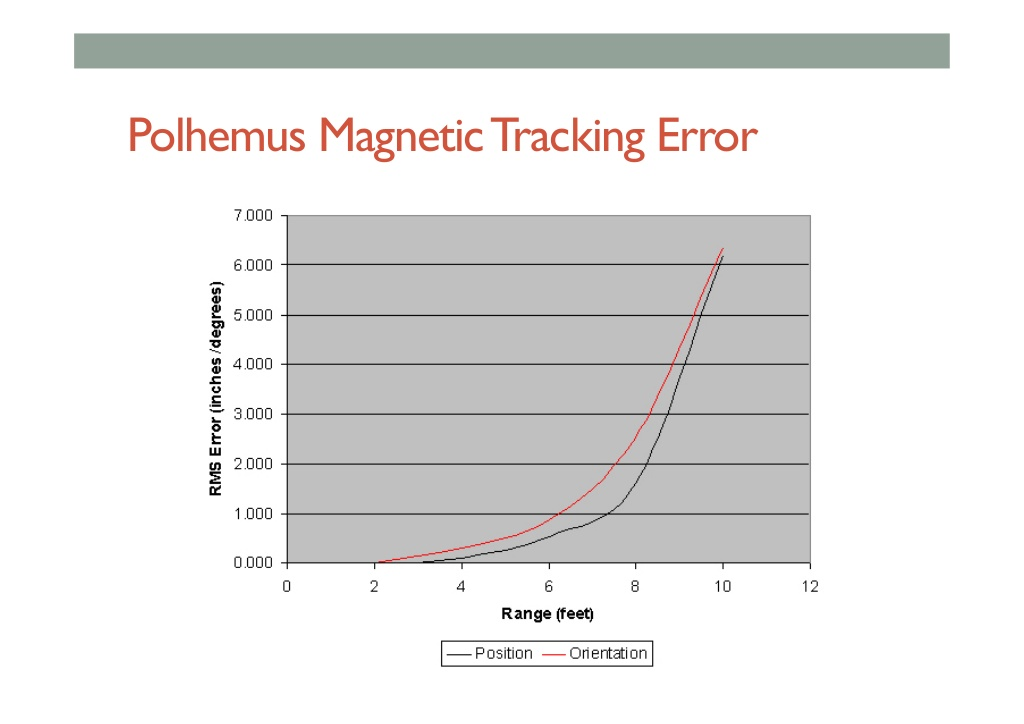
\includegraphics[width=1\linewidth]{image/magnetic}
	\caption {ارتباط فاصله با وضوح محاسبات در ردیابی مغناطیسی\cite{Polhemus}}
	\label{fig:magnetic}
\end{figure}
ردیابی مغناطیسی در طیف وسیعی از سامانه‌های واقعیت افزوده استفاده‌شده است، مانند برنامه‌هایی در حوزه‌های تولید\cite{lhachemi2019augmented}، نگهداری\cite{siew2019practical}، سلامت\cite{ribeiro2019augmented}.
\section{ردیابی براساس دید}
ردیابی بر اساس دید\LTRfootnote{Vision Based Tracking}، یک روش است که شامل ثبت و ردیابی می‌شود درنتیجه در دسته ثبت پویا قرار می‌گیرد و با استفاده از این روش، ما ژست دوربین را با استفاده از گرفتن و پردازش اطلاعاتی که توسط حسگرهای نوری جمع‌آوری می‌شوند، انجام می‌دهیم. این حسگرهای نوری خود به ۳ بخش اصلی تقسیم می‌شوند: حسگرهای مادون‌قرمز\LTRfootnote{Infrared Sensors}، حسگرهای نورهای قابل‌مشاهده\LTRfootnote{Visible Light Sensors} و حسگرهای ساختار ۳ بعدی\LTRfootnote{3D structure sensors}.

ردیابی بر اساس دید، در سیستم‌های واقعیت افزوده بسیار محبوب شده‌اند به دلیل حداقل سخت‌افزارهای موردنیاز، بهبود قدرت محاسباتی دستگاه‌های مشتریان  و همه‌گیر شدن دستگاه‌های قابل‌حمل مانند تلفن‌های همراه و رایانک‌های لوحی\LTRfootnote{tablets} که دارای صفحه‌نمایش و دوربین می‌باشند درنتیجه برای سیستم‌های واقعیت افزوده بسیار ایده آل هستند.

در زیر بخش‌های بعدی در رابطه با حسگرهای مختلف در ردیابی بر اساس دید صحبت می‌کنیم و آن‌ها را بر اساس سخت‌افزاری که استفاده می‌کنند دسته‌بندی می‌کنیم.


\subsection{ردیابی مادون قرمز}
ردیابی مادون قرمز\LTRfootnote{Infrared Tracking}، یکی از اولین روش‌های ردیابی با استفاده از نور بوده است و این روش نورهای منتشرشده و یا بازتاب نور را هدف قرار می‌دهد و به‌راحتی می‌تواند میزان شدت نور را با مقایسه در اطراف محیط به‌دست آورد\cite{bajura1995dynamic}. هدف که نوری را منتشر می‌کند نسبت به اثرات نامطلوب نور مانند نور ضعیف محیط و یا سایه‌ها بسیار مقاوم است. این هدف‌ها همچنین می‌توانند به عنصری که قصد داریم با استفاده از دوربین آن را ردیابی بکنیم وصل بشوند، به این روش نگاه کردن بیرون از داخل\LTRfootnote{outside-looking-in} \cite{ribo2001new}گفته می‌شود و یا در محیط‌های بیرونی که دوربین به هدف وصل شده است با عنوان نگاه کردن داخل از بیرون\LTRfootnote{inside-looking-out} شناخته می‌شود\cite{gottschalk1993autocalibration}. 

با مقایسه حسگرها به این نتیجه رسیده‌ایم که با پیکربندی نگاه کردن درون از بیرون، برای تشخیص جهت بسیار بهتر از پیکربندی نگاه کردن بیرون از درون عمل می‌کند. بسیاری از سیستم‌ها با استفاده از پیکربندی نگاه کردن درون از بیرون  توسعه‌یافته‌اند. به‌طورمعمول یک نمایشگر ثبت‌شده بر روی سر  به همراه یک دوربین  خارجی است و ال‌ئی‌دی های مادون‌قرمز بر روی سقف نصب‌شده‌اند شکل\ref{fig:infrared}. با استفاده از الگوهایی که میدانیم و اطلاعاتی که از ال‌ئی‌دی\LTRfootnote{Light-Emitting Diode (LED)} ها دریافت می‌کنیم، موقعیت و جهت سر کاربر را می‌توانیم تشخیص بدهیم\cite{welch1999hiball}.
\begin{figure}
	\centering
	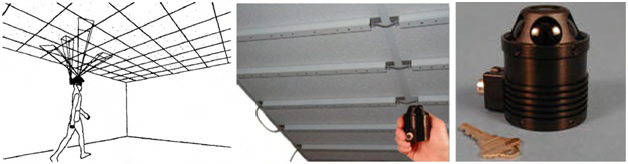
\includegraphics[width=1\linewidth]{image/infrared}
	\caption {چپ: شمایی نمادین از نگاه کردن درون از بیرون-وسط: ال‌ئی‌دی های نصب شده بر روی سقف-راست: ردیاب دوربین\cite{welch1999hiball}}
	\label{fig:infrared}
\end{figure}

مشکل اصلی در پیکربندی نگاه کردن درون از بیرون، نیاز به نصب ال‌ائی‌دی ها در تمام محیط بیرون است و همچنین باید بر روی دستگاه نمایشگر، حسگرهایی برای تشخیص به دوربین موبایل اضافه بشوند که وزن قابل‌توجه ای دارند همچنین این حسگرها بسیار گران و پیچیده هستند.

\subsection{ردیابی نور قابل مشاهده}

رایج‌ترین نوع حسگرهای نوری، حسگرهای نور مرئی هستند و در بسیاری از دوربین‌ها مانند دوربین‌های رایانه‌ها، تلفن‌های همراه و رایانک‌های لوحی می‌توان این حسگرها را پیدا کرد. برای سیستم‌های واقعیت افزوده که از فناوری دیدن از طریق ویدئو استفاده می‌کنند این سنسورها در هر دو حالت ضبط فیلم دنیای واقعی و نیز ثبت عناصر مجازی بر روی دنیای واقعی می‌توانند بسیار مفید واقع شوند.

رروش‌های ردیابی نور قابل مشاهده\LTRfootnote{Visible Light Tracking} که در سنسورهای مخصوص به خود استفاده می‌شوند، می‌توانند به سه دسته تقسیم بشوند. ردیابی ثابت\LTRfootnote{Fiducial tracking}، ردیابی ویژگی‌های طبیعی\LTRfootnote{Natural Feature tracking}، ردیابی بر اساس مدل\LTRfootnote{Model Based tracking}. در ادامه به توضیح هرکدام می‌پردازیم.

	\subsubsection{ردیابی ثابت}
	
در این مدل، ما نشانه‌های ساختگی ثابتی را در نظر می‌گیرم و آن‌ها را  برای ثبت کردن و ردیابی به محیط می‌دهیم\ref{fig:fiducial}. با توجه به برنامه و تکنولوژی که استفاده می‌کنیم پیچیدگی و گسترگی ثابت‌ها می‌توانند متفاوت باشند. در سیستم‌های اولیه از ال ئی دی های رنگی کوچک و یا تکه‌های کاغذ استفاده‌شده است که می‌توانستیم به محیط اضافه بکنیم و با استفاده از تطبیق رنگ آن‌ها را شناسایی بکنیم. اگر درصحنه دریافت شده توسط دوربین بتوانیم به‌اندازه کافی ثابت‌ها را شناسایی بکنیم، ژست دوربین قابل‌شناسایی است. از مزایای این روش می‌توان گفت که در اینجا محیط می‌تواند پویا باشد و برای پیدا کردن ژست دوربین فقط نیاز داریم که ثابت‌ها به محیط در زمان اجزا اضافه بشوند و با کمک آن‌ها موقعیت و جهت دوربین تشخیص داده می‌شود. با اضافه کردن خواص و پیچیدگی به ثابت‌ها مانند چند حلقه‌ای، می‌توان ثابت‌ها را در فواصل بیشتر نیز تشخیص داد شکل \ref{fig:fiducial}\cite{basiratzadeh2019fiducial}.
	
	\begin{figure}
		\centering
		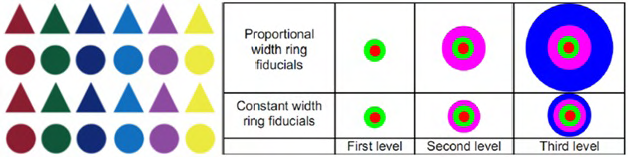
\includegraphics[width=1\linewidth]{image/fiducial}
		\caption {چپ:نشانه های رنگی ثابت-راست: استفاده از چند حلقه به ثابت‌ها\cite{basiratzadeh2019fiducial}}
		\label{fig:fiducial}
	\end{figure}
	برای محاسبه موقعیت یک تماشاگر در دنیای واقعی حداقل باید 4 نقطه از موقعیت‌ها را داشته باشیم و بدانیم. با استفاده از این ثابت‌های ساده، طراحی فضا به‌دقت باید موردتوجه قرار گیرد تا اطمینان حاصل شود که نقاط کافی در هرلحظه قابل‌مشاهده است اگر نیازهای ما برطرف نشد و نیاز به تلاش بیشتر داشتیم، باید توجه شود که می‌توان ثابت‌های بیشتری را به محیط اضافه کرد و باید موقعیت آن‌ها را در محیط به‌صورت دقیق داشته باشیم. یک راه جایگزین که دیگر نیازی به استفاده از چهار نقطه نباشد، این است که از ثابت‌های مسطح به شکل مربع که ۴ گوشه آن می‌تواند برای ما به‌عنوان چهار نقطه‌ای که باید موقعیت آن‌ها را بدانیم عمل کند.
	
	سپس اطلاعات شناسایی اضافی که برای عملیات ثبت نیاز داریم، می‌تواند درون این مربع قرار بگیرد. با این روش می‌توان از چندین ثابت یکتا مختلف در یک برنامه استفاده کرد.
	
	استفاده از ثابت‌های مربعی  به خاطر راحتی در استفاده و نیز دقت بالا در تشخیص بسیار در فنّاوری واقعیت افزوده محبوب شد. یکی از محبوب‌ترین سیستم‌های ثابت‌های مربعی، ARToolkit است که تعداد بسیار زیادی پروژه موفق داشت و توانسته محبوب‌ترین ثابت‌ها را در دنیا ارائه بدهد\cite{ma2019projected}.انواع قالب ثابت‌های ارائه شده توسط  شرکت‌های مختلف در شکل \ref{fig:ARtoolkit} ارائه شده است.
	
		\begin{figure}
		\centering
		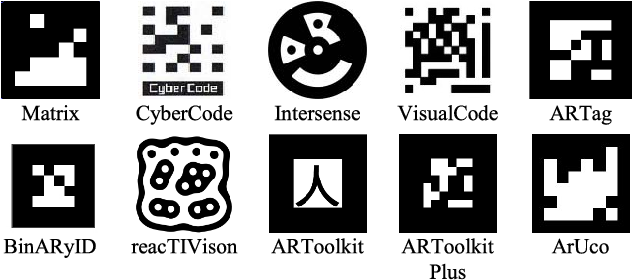
\includegraphics[width=1\linewidth]{image/ARtoolkit}
		\caption {نمونه‌های مختلف ثابت‌های استفاده‌شده  \cite{fiducial}}
		\label{fig:ARtoolkit}
	\end{figure}
	
	\subsubsection{ردیابی ویژگی‌های طبیعی}
	
	ثابت‌های مربعی توانستند مشکلاتی که در ثابت‌های رنگی بود را رفع کنند ولی هنوز مشکلات مربوط به خود رادارند، یکی از این مشکلات این است که نیاز دارند تا شکل محیط را تغییر بدهند که این کار ممکن است مطلوب و یا غیرممکن باشد، مخصوصاً وقتی‌که لنگر برای ما باارزش است مانند یک نقاشی هنری که نمی‌توانیم به آن عنصری را اضافه بکنیم.
	
	با توجه به افزایش قدرت دستگاه‌های استفاده‌شده برای فنّاوری واقعیت افزوده، امکان ثبت ژست دوربین به شکل بلادرنگ با توجه به‌ویژگی‌های طبیعی در محیط امکان‌پذیر است.
	
	برای تشخیص ویژگی‌های منحصربه‌فردی که در محیط عکس‌های گرفته‌شده وجود دارد، مانند نقطه‌ها، گوشه‌ها و تقاطع خطوط، از الگوریتم‌های پردازش تصویر پیچیده استفاده می‌شود.
	
	برای هر یک از ویژگی‌های نام‌برده شده یک "توصیفگر"\LTRfootnote{descriptor} محاسبه‌شده است که برای شناسایی و تفکیک این ویژگی‌ها به‌کار می‌رود. با تطابق دادن ویژگی‌های به‌دست‌آمده از درون صحنه، با ویژگی‌هایی که از عنصری که می‌خواهیم ردیابی بکنیم، سپس می‌توانیم با استفاده از الگوریتم‌های ساده که درروش ردیابی ثابت استفاده کرده‌ایم، ژست را تشخیص بدهیم\cite{gottl2018efficient}.
		\begin{figure}
		\centering
		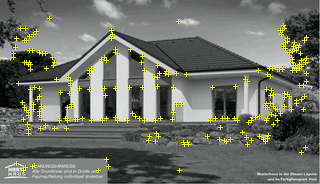
\includegraphics[width=1\linewidth]{image/nft}
		\caption {نمونه‌ای از ردیابی بر اساس ویژگی‌های طبیعی   \cite{nft}}
		\label{fig:nft}
	\end{figure}
	\subsubsection{ردیابی براساس مدل}
	
اگرچه مدل‌های ردیابی بر اساس ثابت و ویژگی‌های طبیعی خیلی محبوب هستند، اما تلاش‌ها برای اینکه بتوانیم ردیابی را بر اساس ویژگی‌های ۳ بعدی عناصر در دنیای واقعی انجام بدهیم بسیار موردتوجه است. این روش‌ها معمولاً به‌صورت ابتکاری هستند و در آن‌ها سعی شده است اجسام را بر اساس مدل ۳ بعدی آن‌ها شناسایی بکنیم و برای این کار از ترکیب ویژگی‌هایی مانند خط‌ها، دایره‌ها، استوانه‌ها و کره‌ها استفاده می‌شود\cite{comport2003real}. در این روش با استفاده از  فیلتر کردن بر اساس ضلع‌ها و استخراج اطلاعات ساختاری عناصر از روی صحنه و تطبیق دادن این اطلاعات با مدل‌های اولیه، برای فهمیدن ژست بکار می‌رود\cite{zubizarreta2019framework}.نمونه‌ای از ردیابی براساس مدل را در شکل \ref{fig:opentl} می‌توان مشاهده نمود.
	
	برای به‌دست آوردن ردیابی قوی‌تر\LTRfootnote{robustness} می‌توانیم ۲ روش ردیابی ویژگی‌های طبیعی و ردیابی بر اساس ضلع‌ها را با یکدیگر ترکیب کنیم\cite{vacchetti2003fusing} و همچنین با این ترکیب می‌توانیم در فضاهای باز و محیط‌های بیرون عمل ردیابی را انجام دهیم\cite{ma2019projected}.
	\begin{figure}
		\centering
		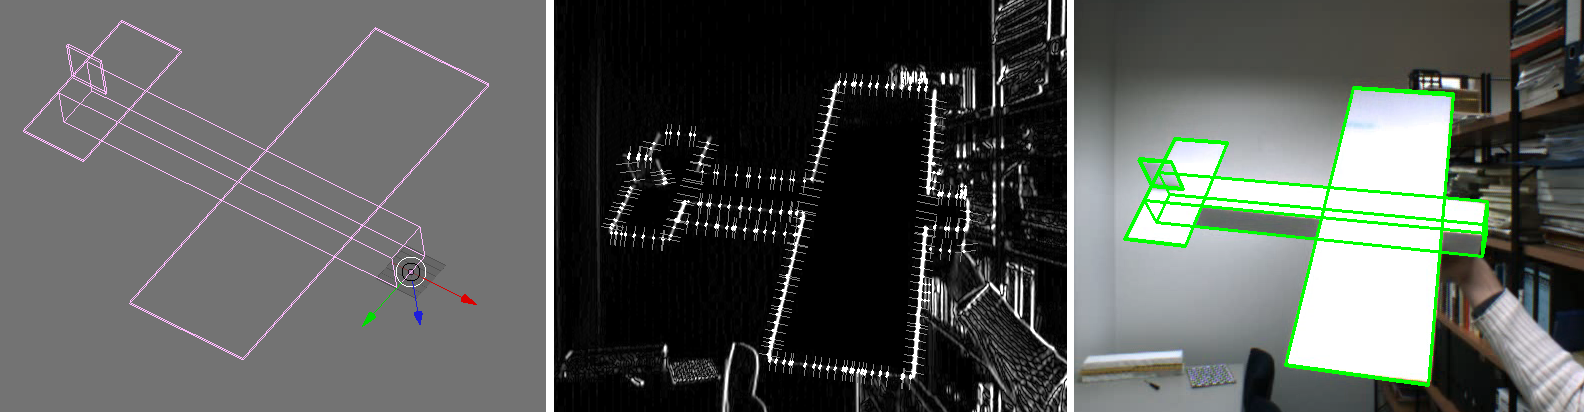
\includegraphics[width=1\linewidth]{image/mbt}
		\caption {نمونه‌ای از ردیابی بر اساس مدل توسط شرکت OpenTL   \cite{mbt}}
		\label{fig:opentl}
	\end{figure}
	اخیراً توجه زیادی شده است که بتوانیم روشی داشته باشیم تا با استفاده از آن ما را قادر سازد به‌صورت همزمان یک نقشه از محیط واقعی را بسازیم و آن را به‌روزرسانی کنیم، و با استفاده از آن بتوانیم موقعیت را تشخیص بدهیم. ایده اصلی این کار با استفاده از روش "مکان‌یابی همزمان و ساختن نقشه "\LTRfootnote{SLAM (Simultaneous Localization and Map Building)} است که این روش اولین بار برای روبات‌ها طراحی شد\cite{dissanayake2001solution} و به آن‌ها راهنمایی می‌کند که چگونه مسیر خودشان را در محیط‌های ناشناخته پیدا بکنند. این روش برای سیستم‌های واقعیت افزوده سازگار شد و با کمک آن کاربر با استفاده از واقعیت افزوده می‌تواند در محیط‌های ناشناخته به مسیریابی بپردازد. همچنین این روش بهینه‌سازی شد و بانام "ردیابی و نقشه‌برداری همزمان "(PTAM)\LTRfootnote{Parallel Tracking and Mapping} شناخته شد(شکل \ref{fig:ptam}) که در آن ردیابی دوربین و نقشه‌برداری به‌صورت جدا از هم کار می‌کردند. PTAM به‌صورت مخصوص فقط برای واقعیت افزوده طراحی شد و دقت ردیابی در آن بالا رفت\cite{davison2007monoslam}.
		\begin{figure}
		\centering
		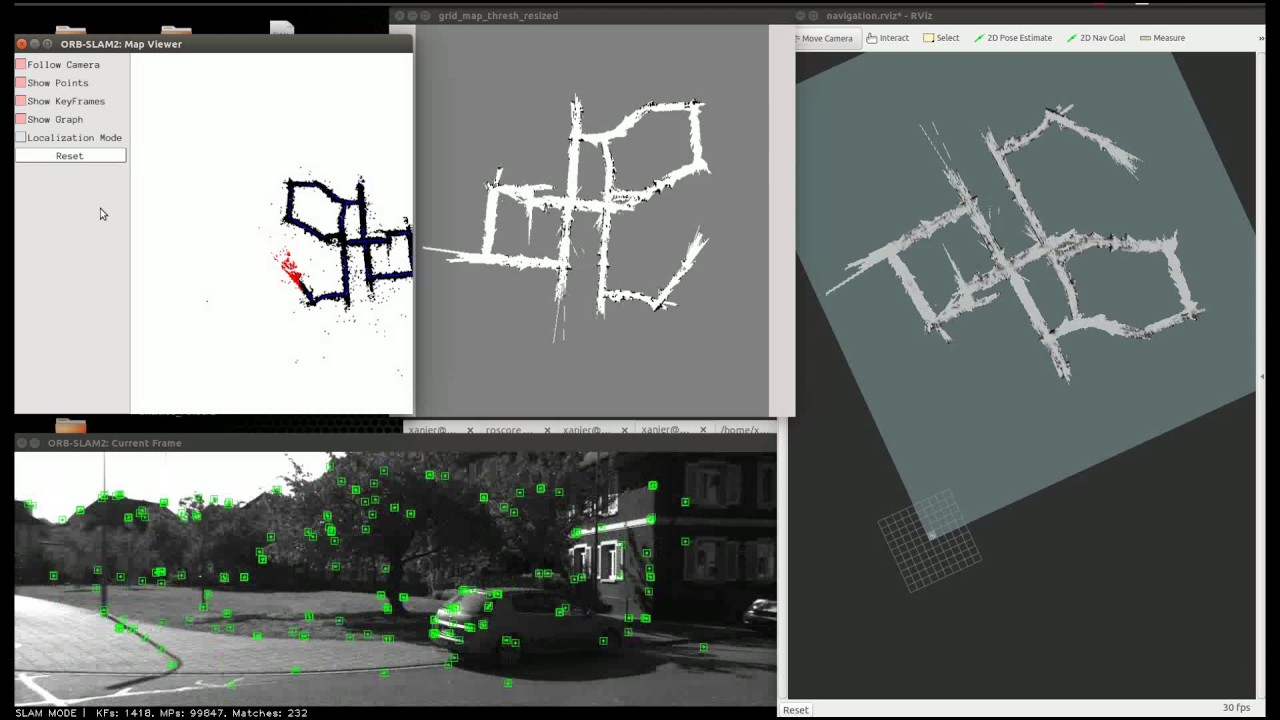
\includegraphics[width=1\linewidth]{image/ptam}
		\caption {نمونه‌ای از روش PTAM    \cite{murORB2}}
		\label{fig:ptam}
	\end{figure}
	


\subsection{ردیابی ساختارهای ۳ بعدی}
در سال‌های اخیر حسگرهای تجاری زیادی به بازار ارائه شدند که توانایی تشخیص ساختار ۳ بعدی از محیط را دارا بودند و همچنین بسیار مقرون‌به‌صرفه بودند، از نمونه‌های اولیه آن‌ها می‌توان به ماکروسافت کینکت\LTRfootnote{Microsoft Kinect} اشاره کرد که شروع‌کننده این حسگرها بود\cite{zhang2012microsoft}. این حسگرها از تکنولوژی‌هایی مانند ساختار نور\cite{scharstein2003high} و یا زمان گریز\LTRfootnote{time-of-flight} \cite{gokturk2004time}برای به‌دست آوردن اطلاعات در مورد موقعیت‌های ۳ بعدی از نقاط درون صحنه استفاده می‌کنند.برای ردیابی ساختارهای ۳ بعدی\LTRfootnote{3D Structure Tracking} از این حسگرها استفاده می‌شود.
\begin{figure}
	\centering
	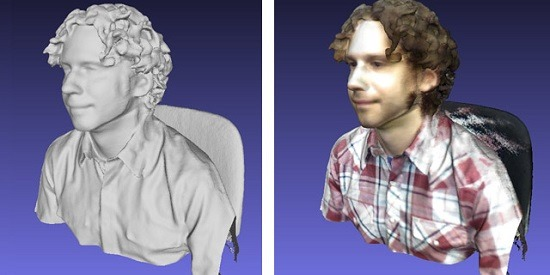
\includegraphics[width=1\linewidth]{image/kinect}
	\caption {نمونه‌ای از ردیابی ساختارهای ۳ بعدی توسط کینکت ماکروسافت    \cite{izadi2011kinectfusion}}
	\label{fig:kinect}
\end{figure}

 این فنّاوری‌های جدید، فرصت‌های جدیدی را برای ردیابی و نقشه‌برداری از محیط واقعی را با استفاده از اطلاعات عمق ایجاد کردند. بیشترین رویکردی که برای سیستم‌های واقعیت افزوده استفاده می‌شود در حال حاضر کینکت فیوژن\LTRfootnote{KinectFusion} است که توسط شرکت ماکروسافت توسعه‌یافته است. کینکت فیوژن از اطلاعات به‌دست‌آمده توسط سنسور عمق نور ساختار کینکت استفاده می‌کند تا باکیفیت بالا مدلی ۳ بعدی از عناصر واقعی و محیط به‌دست آورد و از این مدل برای ردیابی ژست کینکت در محیط استفاده می‌کند. شکل \ref{fig:kinect} مثالی از کینکت فیوژن را نشان می‌دهد\cite{izadi2011kinectfusion}.

\section{ردیابی درونی}

ردیابی درونی\LTRfootnote{Inertial Tracking} از (واحد اندازه‌گیری درونی)\LTRfootnote{Inertial Measurement Unit (IMU)} استفاده می‌کند که شامل حسگرهایی مانند شتاب سنج \LTRfootnote{Accelerometers}، ژیروسکوپ \LTRfootnote{Gyroscopes} و مغناطیس‌سنج \LTRfootnote{Magnetometers} است که ابزارهای اندازه‌گیری خوانده می‌شوند، برای اندازه‌گیری جهت نسبی و سرعت وسیله موردنظر از این حسگرها استفاده می‌کنیم. این ابزارها با استفاده از جاذبه و تغییرات در سرعت جسم، جهت نسبی و مکان وسیله را اندازه‌گیری می‌کنند. معمولاً این نوع سنسورها در طول زمان دچار خطا می‌شوند و باعث ایجاد خطا در اندازه‌گیری مکان و جهت می‌شوند. به همین دلیل در کاربردهایی که نیاز به‌دقت بالای ردیابی دارند، نیاز است این روش با روش‌های مبتنی بر دید و یا دیگر روش‌های معرفی‌شده ترکیب شود\cite{Billinghurst}.
\section{ردیابی براساس سیستم موقعیت‌یاب جهانی}
تکنولوژی سیستم موقعیت‌یاب جهانی اجازه ردیابی موقعیت را در محیط‌های بیرونی در بیشتر سطح کره زمین به ما می‌دهد. دقت متوسط سیستم موقعیت‌یاب جهانی حدود ۳ متر می‌باشد و با پیشرفت‌های صورت گرفته درون فنّاوری ماهواره‌ها، رو به بهبود است.
ردیابی بر اساس سیستم موقعیت‌یاب جهانی\LTRfootnote{GPS Tracking}، در بسیاری از برنامه‌ها بکار رفته است ازجمله برنامه‌های نظامی، بازی و یا تاریخی. 

باید توجه داشت در این مدل از ردیابی، دقت پایین است و فقط با کمک آن می‌توان موقعیت را ردیابی کرد و نسبت به جهت هیچ حرفی نمی‌توان زد بااین‌وجود در برنامه‌هایی که دقت برای ما از اهمیت کمتری برخوردار است و یا برنامه‌هایی که از ردیابی ترکیبی استفاده می‌کنند، می‌توان از این مدل ردیابی استفاده نمود\cite{rajeev2019augmented}.برای نام بردن از برنامه‌ای که از این تکنولوژی به صورت ترکیبی استفاده کرده است می‌توان به پوکمون گو\LTRfootnote{pokemon go} اشاره نمود که در شکل \ref{fig:pokemongo} می‌توان نمایی از این برنامه را دید.

\begin{figure}
	\centering
	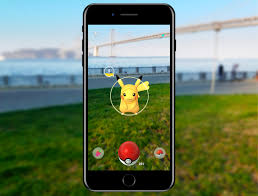
\includegraphics[width=1\linewidth]{image/pokemongo}
	\caption {پوکمون گو نمونه‌ای از برنامه‌هایی که درروش ترکیبی از ردیابی بر اساس سیستم موقعیت‌یاب جهانی استفاده کرده است    \cite{pokemongo}}
	\label{fig:pokemongo}
\end{figure}

\section{ردیابی ترکیبی}
ردیابی ترکیبی\LTRfootnote{Hybrid Tracking}، اطلاعات به‌دست‌آمده از چند حسگر را با یکدیگر ترکیب می‌کند و باعث می‌شود دقت به نسبت اطلاعات به‌دست‌آمده از یک حسگر بالاتر رود و همچنین مشکلات موجود در بعضی از روش‌های گفته‌شده را پوشش می‌دهد\cite{isham2018framework}.

اغلب برنامه‌هایی که بر اساس ردیابی نوری هستند، از ردیابی مغناطیسی و یا ردیابی درونی نیز استفاده می‌کنند. این کار به سیستم اجازه می‌دهد تا نوسانات حاصل از ردیابی نوری را کمتر بکند. هنگامی‌که حسگرهایی با نرخ به‌روزرسانی بالا و باقابلیت اطمینان بالا استفاده شوند می‌توانند مشکلات به‌روزرسانی گرافیک را برطرف بکنند و نیز باعث بالا رفتن دقت در محاسبات ژست بشوند.
\begin{figure}
	\centering
	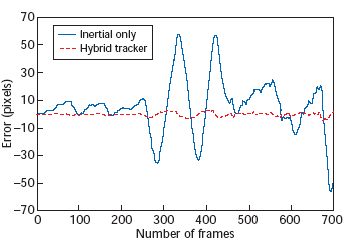
\includegraphics[width=1\linewidth]{image/hybrid}
	\caption {مقایسه سیستم ترکیبی\cite{you1999orientation}}
	\label{fig:hybrid}
\end{figure}

به‌عنوان یک مزیت دیگر می‌توان به این نکته اشاره کرد که ردیابی‌های مغناطیسی و درونی، فاقد خط دید هستند و از آن‌ها برای بالا بردن محدوده استفاده از واقعیت افزوده می‌توان استفاده کرد. 

همان‌طور که در شکل \ref{fig:hybrid} می‌بینیم، با استفاده از ردیابی ترکیبی دقت بسیار بالاتر آمده است\cite{you1999orientation}.

به خاطر دقت پایین و فاقد جهت بودن در ردیابی بر اساس سیستم موقعیت‌یاب جهانی، این نوع ردیابی در بیشتر موارد با ردیابی‌های دیگر ترکیب می‌شود.

در دستگاه‌های قابل‌حمل مانند تلفن‌های همراه و یا رایانک های لوحی، فرصت‌های جدیدی برای استفاده از ردیابی ترکیبی به‌دست آمد. بسیاری از این دستگاه‌ها شامل دوربین، شتاب سنج، ژیروسکوپ، سیستم موقعیت‌یاب جهانی و شبکه بدون سیم هستند که به ردیابی ترکیبی بسیار کمک می‌کند. یکی از مشکلات سیستم موقعیت‌یاب جهانی، استفاده از آن درون ساختمان‌ها است که با استفاده از شبکه بی‌سیم می‌توان به موقعیت‌یابی آن کمک کرد و دقت را بالا برد\cite{duan2018augmented}.
\section{خلاصه}
در این بخش ما روش‌های گوناگون ردیابی در واقعیت افزوده را شرح دادیم که با کمک آن‌ها سعی می‌شود تا عناصر مجازی در دنیای واقعی قرار بگیرند. در جدول \ref{tab:trackingtab} به خلاصه مزیت‌ها و معایب هر یک از روش‌ها آورده شده است.
با توجه به معایب روش‌ها، برای داشتن سیستم واقعیت افزوده قابل‌اعتماد، نیاز داریم تا از روش ترکیبی استفاده بکنیم و معایب هر روش را با استفاده از روشی دیگر بپوشانیم.

\cchapter{نتیجه گیری و کارهای آینده}
% Please add the following required packages to your document preamble:
% \usepackage{booktabs}
\begin{table}
	\centering
\Rotatebox{90}{%
	\scalebox{0.65}{%
	\begin{tabular}{@{}|c|c|c|c|c|@{}}
		\toprule
		روش & محیط & محدوده & مزایا & معایب \\ \midrule
		ردیابی مغناطیسی & درونی و بیرونی & متوسط & دقت بالا در فواصل نزدیک & گران است - با افزایش فاصله دقت بصورت چند جمله‌ای کاهش میابد -حساسیت نسبت به الکترومغناطیس\\ \midrule
		ردیابی مادون قرمز & درونی & کم & دقت بالا & نیاز به آماده سازی محیط دارد \\ \midrule
		ردیابی ثابت & درونی و بیرونی & کم & دقت بالا & نیاز به ایجاد تغییر در لنگر دارد \\ \midrule
		ردیابی ویژگی‌های طبیعی & درونی و بیرونی & کم & دقت بالا & نسبت به تغییرات نور حساس است \\ \midrule
		ردیابی بر اساس مدل & درونی و بیرونی & کم & دقت بالا & فقط برای مدل‌هایی با شباهت بالا کاربرد دارد \\ \midrule
		ردیابی ساختارهای ۳ بعدی & درونی & خیلی کم & تشخیص به صورت ۳ بعد - دقت در فواصل نزدیک خیلی خوب & دقت در فواصل زیاد بد - محوده خیلی کم \\ \midrule
		ردیابی درونی & درونی & خیلی کم & دقت بسیار بالا & محدوده کم - عمر پایین حسگرها \\ \midrule
		ردیابی براساس سیستم موقعیت‌یاب جهانی & بیرونی & زیاد & ردیابی بر روی کل فضای زمین & دقت پایین - عملکرد پایین درون ساختمان‌ها \\ \midrule
		ردیابی ترکیبی & درونی و بیرونی & زیاد & می‌تواند مزایای هر روشی را شامل شود &  \\ \bottomrule
	\end{tabular}

}
}%
\caption{مقایسه روش‌های ردیابی} \label{tab:trackingtab}
\end{table}


دنیای امروز دنیای اطلاعات است و کاربران به دنبال دریافت اطلاعات به روش‌های سریع‌تر و راحت‌تر هستند. واقعیت افزوده فنّاوری است که می‌تواند گامی بزرگ در این رابطه بردارد. 
پس از مطالعه کارهای پیشین، اهمیت موضوع واقعیت افزوده و در کنار آن رندرینگ واضح است، ما قصد داریم در مبحث رندرینگ مطالعات بیشتری انجام داده و نیز تمرکز خود را بر روی ردیابی و روش‌های ترکیبی قرار بدهیم. همان‌طور که در بررسی دو دهه برگزاری کنفرانس ایسمار\cite{ismar} و مقاله‌های ارائه شده در آن آورده شد (شکل \ref{fig:ISMAR})، مسئله ردیابی یکی از مهم‌ترین و پرمخاطب‌ترین حوزه‌ها درون واقعیت افزوده است. برای امکان پذیری حل این مسئله می‌توان گفت روش‌های نام برده شده، همه سعی در برطرف کردن نقص‌های موجود در ردیابی داشته‌اند و سعی بر آن است تا بتوان این روش‌ها را بهبود بخشید. در پایان نامه بعد از مطالعه و بهبود دادن روش‌ها، پیاده سازی نیز خواهیم داشت و برای پیاده سازی از زبان‌های سی\LTRfootnote{C} و همینطور نرم افزار یونیتی\LTRfootnote{Unity} و کتابخانه وفوریا\LTRfootnote{Vuforia} استفاده خواهیم کرد.

همان‌طور که در شکل \ref{fig:ISMAR} آورده شده است، موضوعات داغ در این حوزه شامل ردیابی، تعامل و استفاده از فنّاوری واقعیت افزوده و ارزیابی تاثیرات آن است. همانطور که در رابطه با ردیابی گفته شد، بهترین روش‌ پایه، روش ترکیبی است زیرا با کمک آن می‌توان معایب روش‌های دیگر را پوشاند و برای بالا بردن دقت از این روش استفاده کرد. در رابطه با ضعف‌ها و مزیت‌های روش‌ها، درون جدول \ref{tab:trackingtab} صحبت شده است.

در رابطه با کارهای آینده میتوان گفت تمرکز ما بیشتر بر روی گوشی های موبایل خواهد بود و بررسی بیشتر در زمینه ردیابی ویژگی‌های طبیعی و ردیابی براساس مدل صورت خواهد گرفت و در نتیجه سعی در بهبود رندرینگ بر روی گوشی های موبایل خواهیم کرد.
